\documentclass[a4paper,9pt]{article}
\usepackage[T1]{fontenc}
\usepackage[utf8]{inputenc}
\usepackage[italian]{babel}
\usepackage{graphicx}
\usepackage{subcaption}
\usepackage{caption}
\usepackage{gensymb}
\usepackage{colortbl}
\usepackage{multicol}
\usepackage{wrapfig}
\usepackage{booktabs}
\usepackage{amsmath,bm}
\usepackage{siunitx}
\usepackage{float}
\usepackage{hyperref}
\usepackage{array}
\usepackage{color}
\usepackage{colortbl}
\usepackage{amsmath}
\captionsetup{tableposition=top,figureposition=bottom,font=footnotesize}
\renewcommand{\vec}{\mathbf}
\usepackage{upgreek}
\usepackage[a4paper, total={7.7in, 10.5in}]{geometry}
\begin{document}
\title{Relazione del Progetto di Data Mining}
\title{%
  Relazione del Progetto di Data Mining \\
  \large Corso di Laurea Magistrale in Fisica \\
    Esame di Data Mining A.A. 2020/2021}
\author{Gruppo 33: Daniele Maria Di Nosse, Angelo Lasala, Raffaele Paradiso}
\maketitle
\newpage

\maketitle
\tableofcontents{}

\newpage

\section{Introduzione}
Determinare le possibili relazioni che intercorrono fra le caratteristiche dei dipendenti di un'azienda può risultare di grande utilità per predire i possibili scenari lavorativi che posso verificarsi e gestire di conseguenza l'organizzazione del personale in maniera ottimale. Nel presente progetto ci si è posto l'obiettivo di valutare tali legami tramite un approccio di data mining. Le informazioni che si sono utilizzate sono relative ad un data frame fittizio (leggermente modificato) generato da IBM e presente sul portale Kaggle(URL \url{https://www.kaggle.com/pavansubhasht/ibm-hr-analytics-attrition-dataset}). Non ci si è posto un obiettivo principale, ovvero la determinazione di legami, correlazioni e classificazioni relativi ad un singolo attributo rispetto a tutti gli altri, ma si è proceduto in maniera più generale ricoprendo uno spettro più ampio di possibili relazioni fra tutte le variabili.
\section{Data Understanding}
\subsection{Data Semantics}
Nella prima fase dell'elaborazione si è studiato il data frame, valutando il numero degli attributi, la loro natura e dominio. 

%\begin{center}
%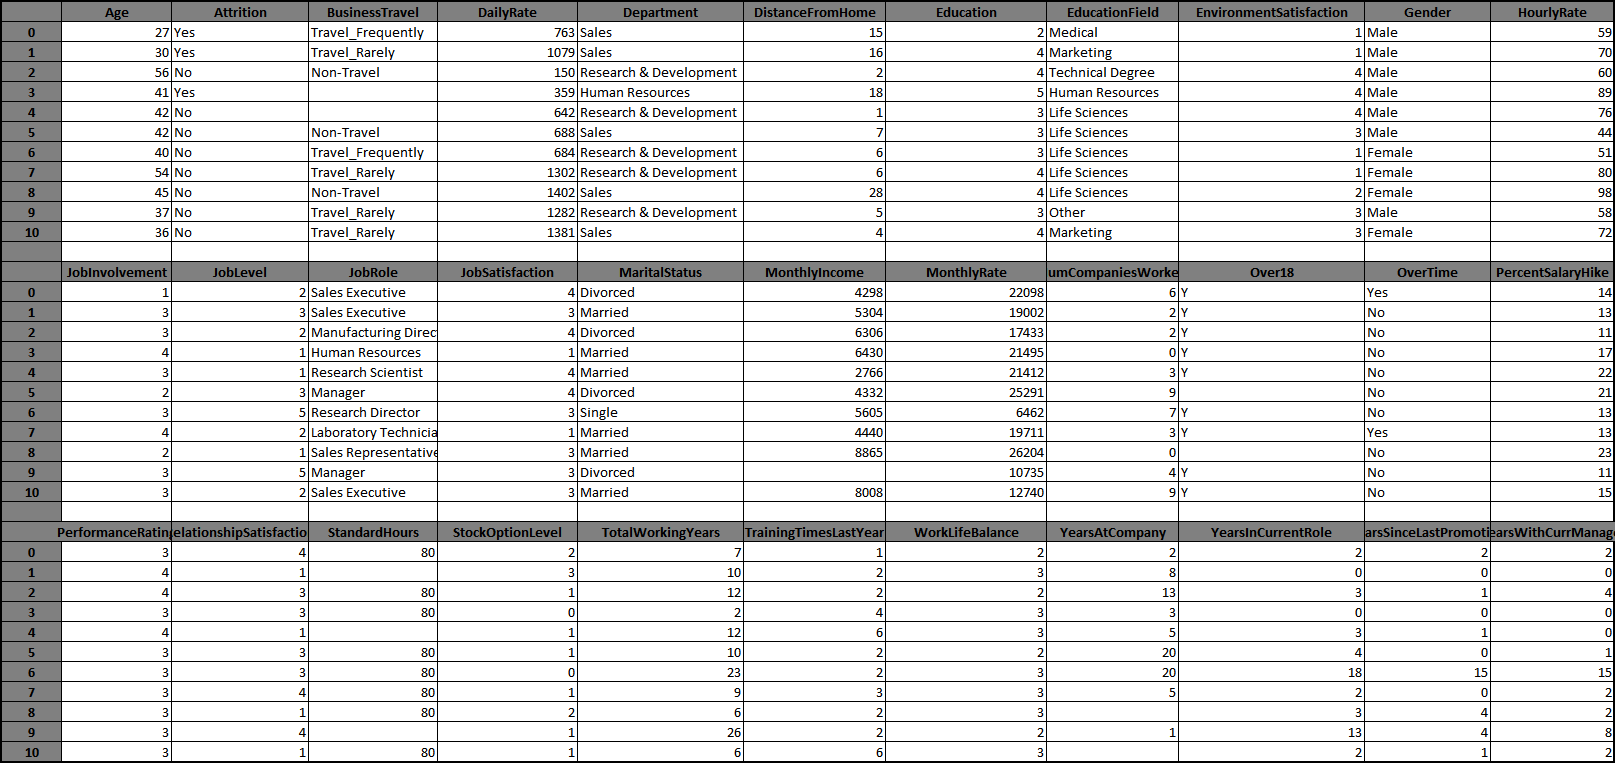
\includegraphics[scale=0.5]{DFhead(10).png}
%\captionof{figure}{Primi 10 valori di ogni attributo}
%\end{center}
% trim=2cm 0 0 0cm

Il numero di attributi è pari a 33. Si dividono in attributi numerici e categorici, ma ad uno sguardo più attento si nota che alcuni di essi, come Education o EnviromentSatisfaction, presentano valori numerici che poco si adattano al loro significato. Si ha infatti che sussistono le seguenti relazioni: 

\begin{center}
\begin{tabular}{l|l|l|l}
\hline
Education & EnvironmentSatisfaction & JobInvolvement & JobSatisfaction \\
\hline
\hline
1 : `Below College' & 1 : `Low'  & 1 : `Low'& 1 : `Low' \\
2 : `College'  & 2 : `Medium' & 2 : `Medium'& 2 : `Medium'\\
3 : `Bachelor'    &3 : `High' & 3 : `High'& 3 : `High'  \\
4 : `Master'    &4 : `Very High' & 4 : `Very High' & 4 : `Very High' \\
5 : `Doctor'  &  & &\\
\hline
\end{tabular}
\end{center}


%\begin{table}{I}{0.7\linewidth}
%\centering
\begin{center}
\begin{tabular}{l|l|l}
\hline
PerformanceRating & RelationshipSatisfaction&WorkLifeBalance \\
\hline
\hline
1 : `Low' & 1 : `Low' & 1 : `Bad'\\
2 : `Good' & 2 : 'Medium'& 2 : `Good'\\
3 : `Excellent'& 3 : `High' & 3 : `Better'\\
4 : `Outstanding'& 4 : `Very High' &4 : `Best'\\
\hline
\end{tabular}
\end{center}

%\end{table}

Di conseguenza, il dominio di tali attributi è di tipo categorico od ordinale e non numerico (un attributo ordinale è effettivamente una sottocategoria categorica, si è scelto comunque di elencarli separatamente). Inoltre, sebbene non si abbiano informazioni dettagliate sulle classi relative agli attributi JobLevel e  StockOptionLevel, per la loro stessa natura si è deciso di trattarli come attributi ordinali. Organizzando tutte le variabili per la loro tipologia, si ottiene quindi la seguente suddivisione:

\begin{center}
\begin{tabular}{c|c|c}
\toprule
\bfseries Categorici: 8 &\bfseries Ordinali: 10 & \bfseries Numerici: 15 \\
\midrule
Attriction & Business Travel & Age \\
Department & Education & Daily Rate \\
Education Filed & Enviroment Satisfaction & Distance From Home \\
Gender & Job Involvement & Monthly Income \\
Job Role & Job Level & Monthly Rate\\
Marital Status & Job Satisfaction & Montly Rate\\
Over 18 & Performance Rating & Num Company Worked\\
Over Time & Relationship Satisfaction & Persent Salary Hike\\
& Stock Option Level & Standard Hours\\
& Work Life Balance & Total Working Years\\
& &Training Time Last Year\\
& & Years At Company\\
& & Years In Current Role\\
& & Years Since Last Promotion\\
& & Yeaer With Current Manager\\
\bottomrule 
\end{tabular}
\end{center}

Per quanto riguarda il range di valori degli attributi risulta essere molto più discretizzato per gli attributi ordinali che per gli attributi numerici. Inoltre differisce molto da attributo ad attributo (anche di 4 ordini di grandezza), cosa che sottolinea sin da  ora l'importanza di una trasformazione delle variabili.

\subsection{Analisi statistica}
Le frequenze degli attributi categorici e le relative mode sono riportate nelle seguenti tabelle.

\begin{center}
\begin{tabular}{lllll}
\toprule
\bfseries Attriction &\bfseries  Educational Field & \bfseries Departement &\bfseries  Gender & \bfseries Over Time\\
\hline
\hline
\rowcolor[gray]{0.9}
`No': $83.9\%$ &`Life Science': $41.2\%$ &` Research and Development': $65.4\%$ & `Male': $57.2\%$ & `No': $71.7\%$ \\
`Yes': $16.1\%$ &`Medical': $31.6\%$ &`Sales': $30.3\%$ & `Female': $37.7\%$ & `Yes': $28.3\%$ \\
\rowcolor[gray]{0.9}
                          &`Marketing': $10.8\%$ &`Human Resources': $4.3\%$ & `MISSING': $5.1\%$ &  \\
                          &`Technical Degree': $9.0\%$ &                                   &                                 &  \\
\rowcolor[gray]{0.9}
                          &`Other': $5.6\%$ &                                   &                                 &  \\
                          &`Human Resources': $1.8\%$ &                                   &                                 &  \\
\end{tabular}
\begin{tabular}{lllll}
\toprule
\bfseries Busniss Travel &\bfseries  Job Rule& \bfseries Marital Status &\bfseries  Over 18 & \\
\hline
\hline
\rowcolor[gray]{0.9}
`Travel Rarely': $64.4\%$ &`Sales Executive': $22.2\%$ &`Married': $45.8\%$ & `Yes': $68.2\%$ &\\
`Travel Frequently': $17.3\%$ &`Research Scientist': $19.9\%$ &`Single': $32.0\%$ & `MISSING': $31.8\%$ &\\
\rowcolor[gray]{0.9}
`Non Travel': $9.4\%$ &`Laboratory Technician': $17.6\%$ &`Divorced': $3.2\%$ &       &      \\
`MISSING': $9.0\%$ &`Manufactoring Derector': $9.9\%$ &     &       &      \\
\rowcolor[gray]{0.9}
                               &`Healthcare Representative': $8.9\%$ &     &       &      \\
                               &`Manager': $6.9\%$ &     &       &      \\
\rowcolor[gray]{0.9}
                               &`Sales Representative': $5.6\%$ &     &       &      \\
                               &`Research Derector': $5.4\%$ &     &       &      \\
\rowcolor[gray]{0.9}
                               &`Human Resources': $3.5\%$ &     &       &      \\
\bottomrule
\end{tabular}
\captionof{figure}{Frequenze degli attributi categorici}
\end{center}


\begin{center}
\begin{tabular}{lc}
\toprule
 &\bfseries Moda \\
\hline
\hline
\rowcolor[gray]{0.9}
Attriction & No\\
Educational Field & Life Science\\
\rowcolor[gray]{0.9}
Departement & Research and Development\\
Gender & Male\\
\rowcolor[gray]{0.9}
Over Time & No\\
Business Travel & Travel Rarely\\
\rowcolor[gray]{0.9}
Job Rule & Sales Executive\\
Marital Status & Married \\
\rowcolor[gray]{0.9}
Over 18 & Yes\\ 
Education & Bachelor\\
\rowcolor[gray]{0.9}
Envirorment Satisfaction & High\\
Job Involvement & High\\
\rowcolor[gray]{0.9}
Job Satisfaction & Very High\\
Performance Rating & Excellent\\
\rowcolor[gray]{0.9}
Relationship Satisfaction & High\\
Job Level & 1\\
\rowcolor[gray]{0.9}
Work Life Balace & Better\\
Stock Option Level & 0\\
\bottomrule 
\end{tabular}
\captionof{figure}{Mode}
\end{center}
 
Le distribuzioni degli attributi ordinali e numerici con alcuni indici statistici sono rappresentate di seguito.
Si può notare la forte asimmetria di molte distribuzioni ed un varianza molto grande in alcuni attributi. Tali problematiche dovranno essere sanate con opportune trasformazioni.

\begin{center}
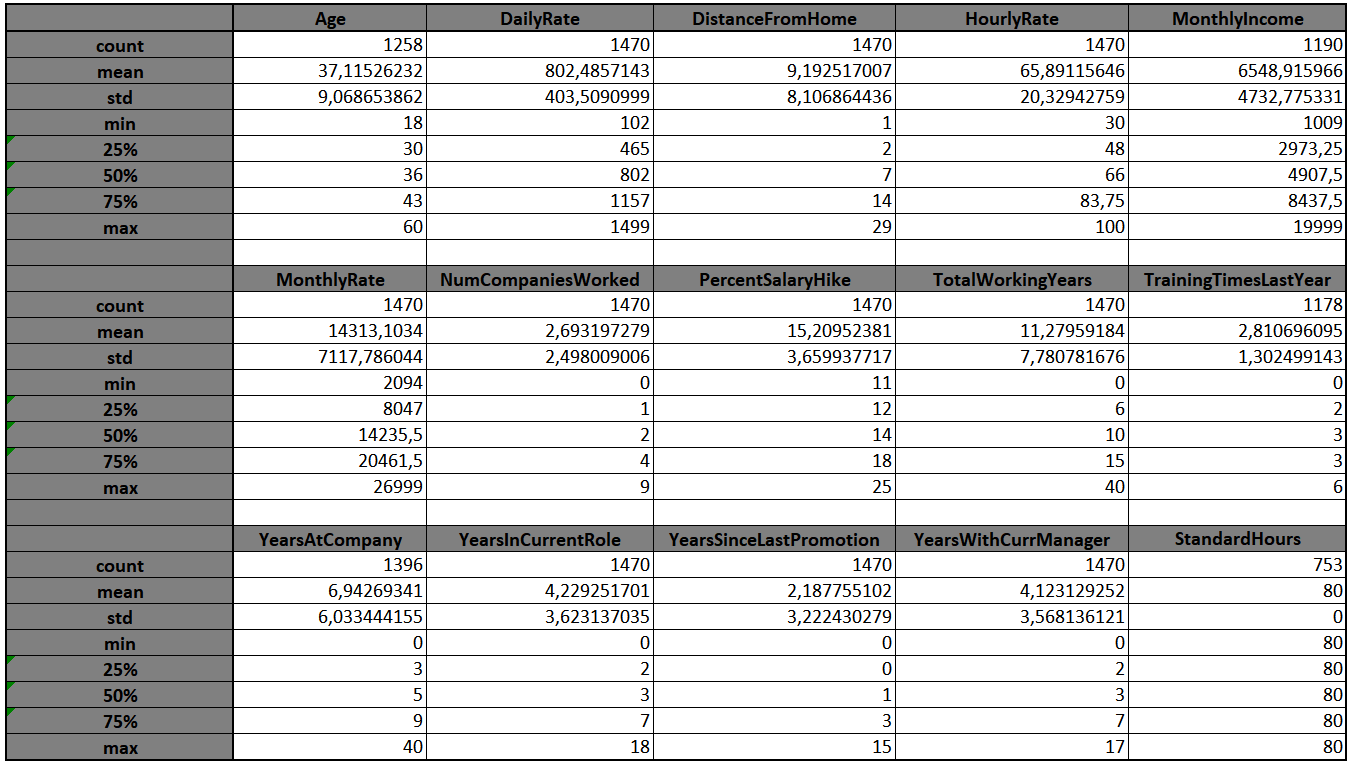
\includegraphics[scale=1.1]{statistica.png}
\captionof{figure}{Indici statistici per gli attributi numerici}
\end{center}

\begin{center}
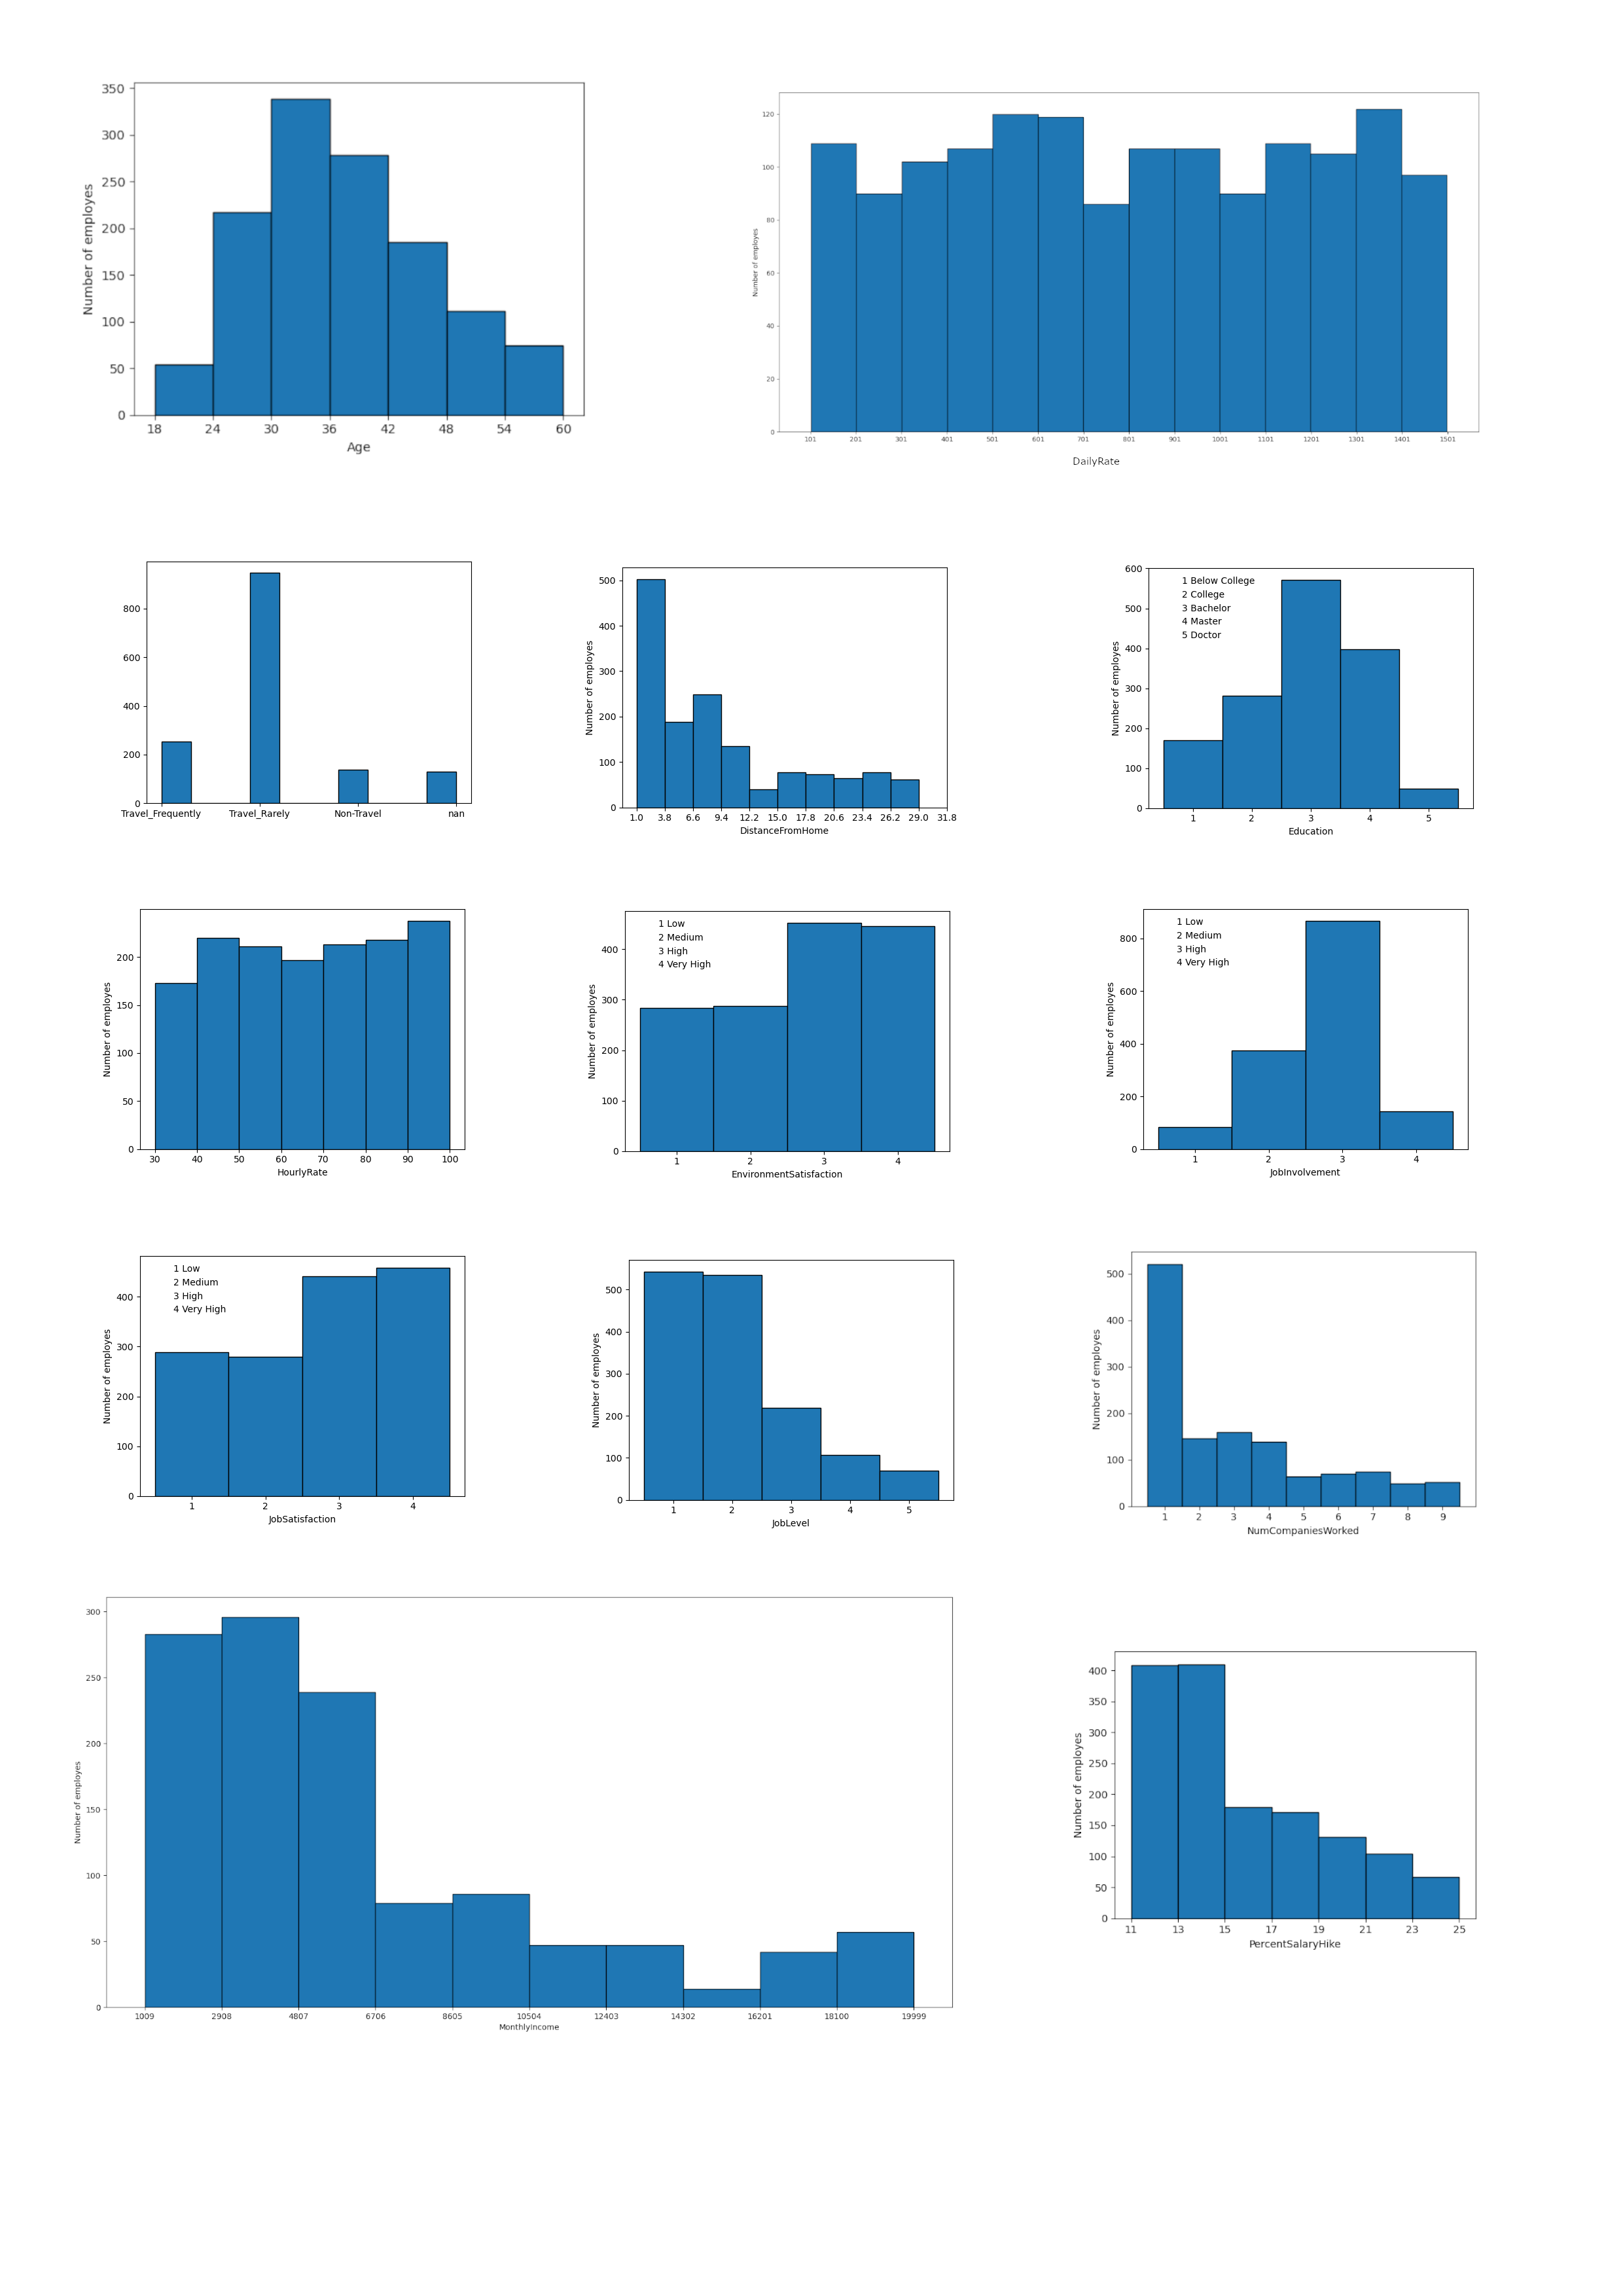
\includegraphics[scale=0.82,trim=0cm 0 0 0cm]{Istogrammi1.png}
\end{center}


\begin{center}
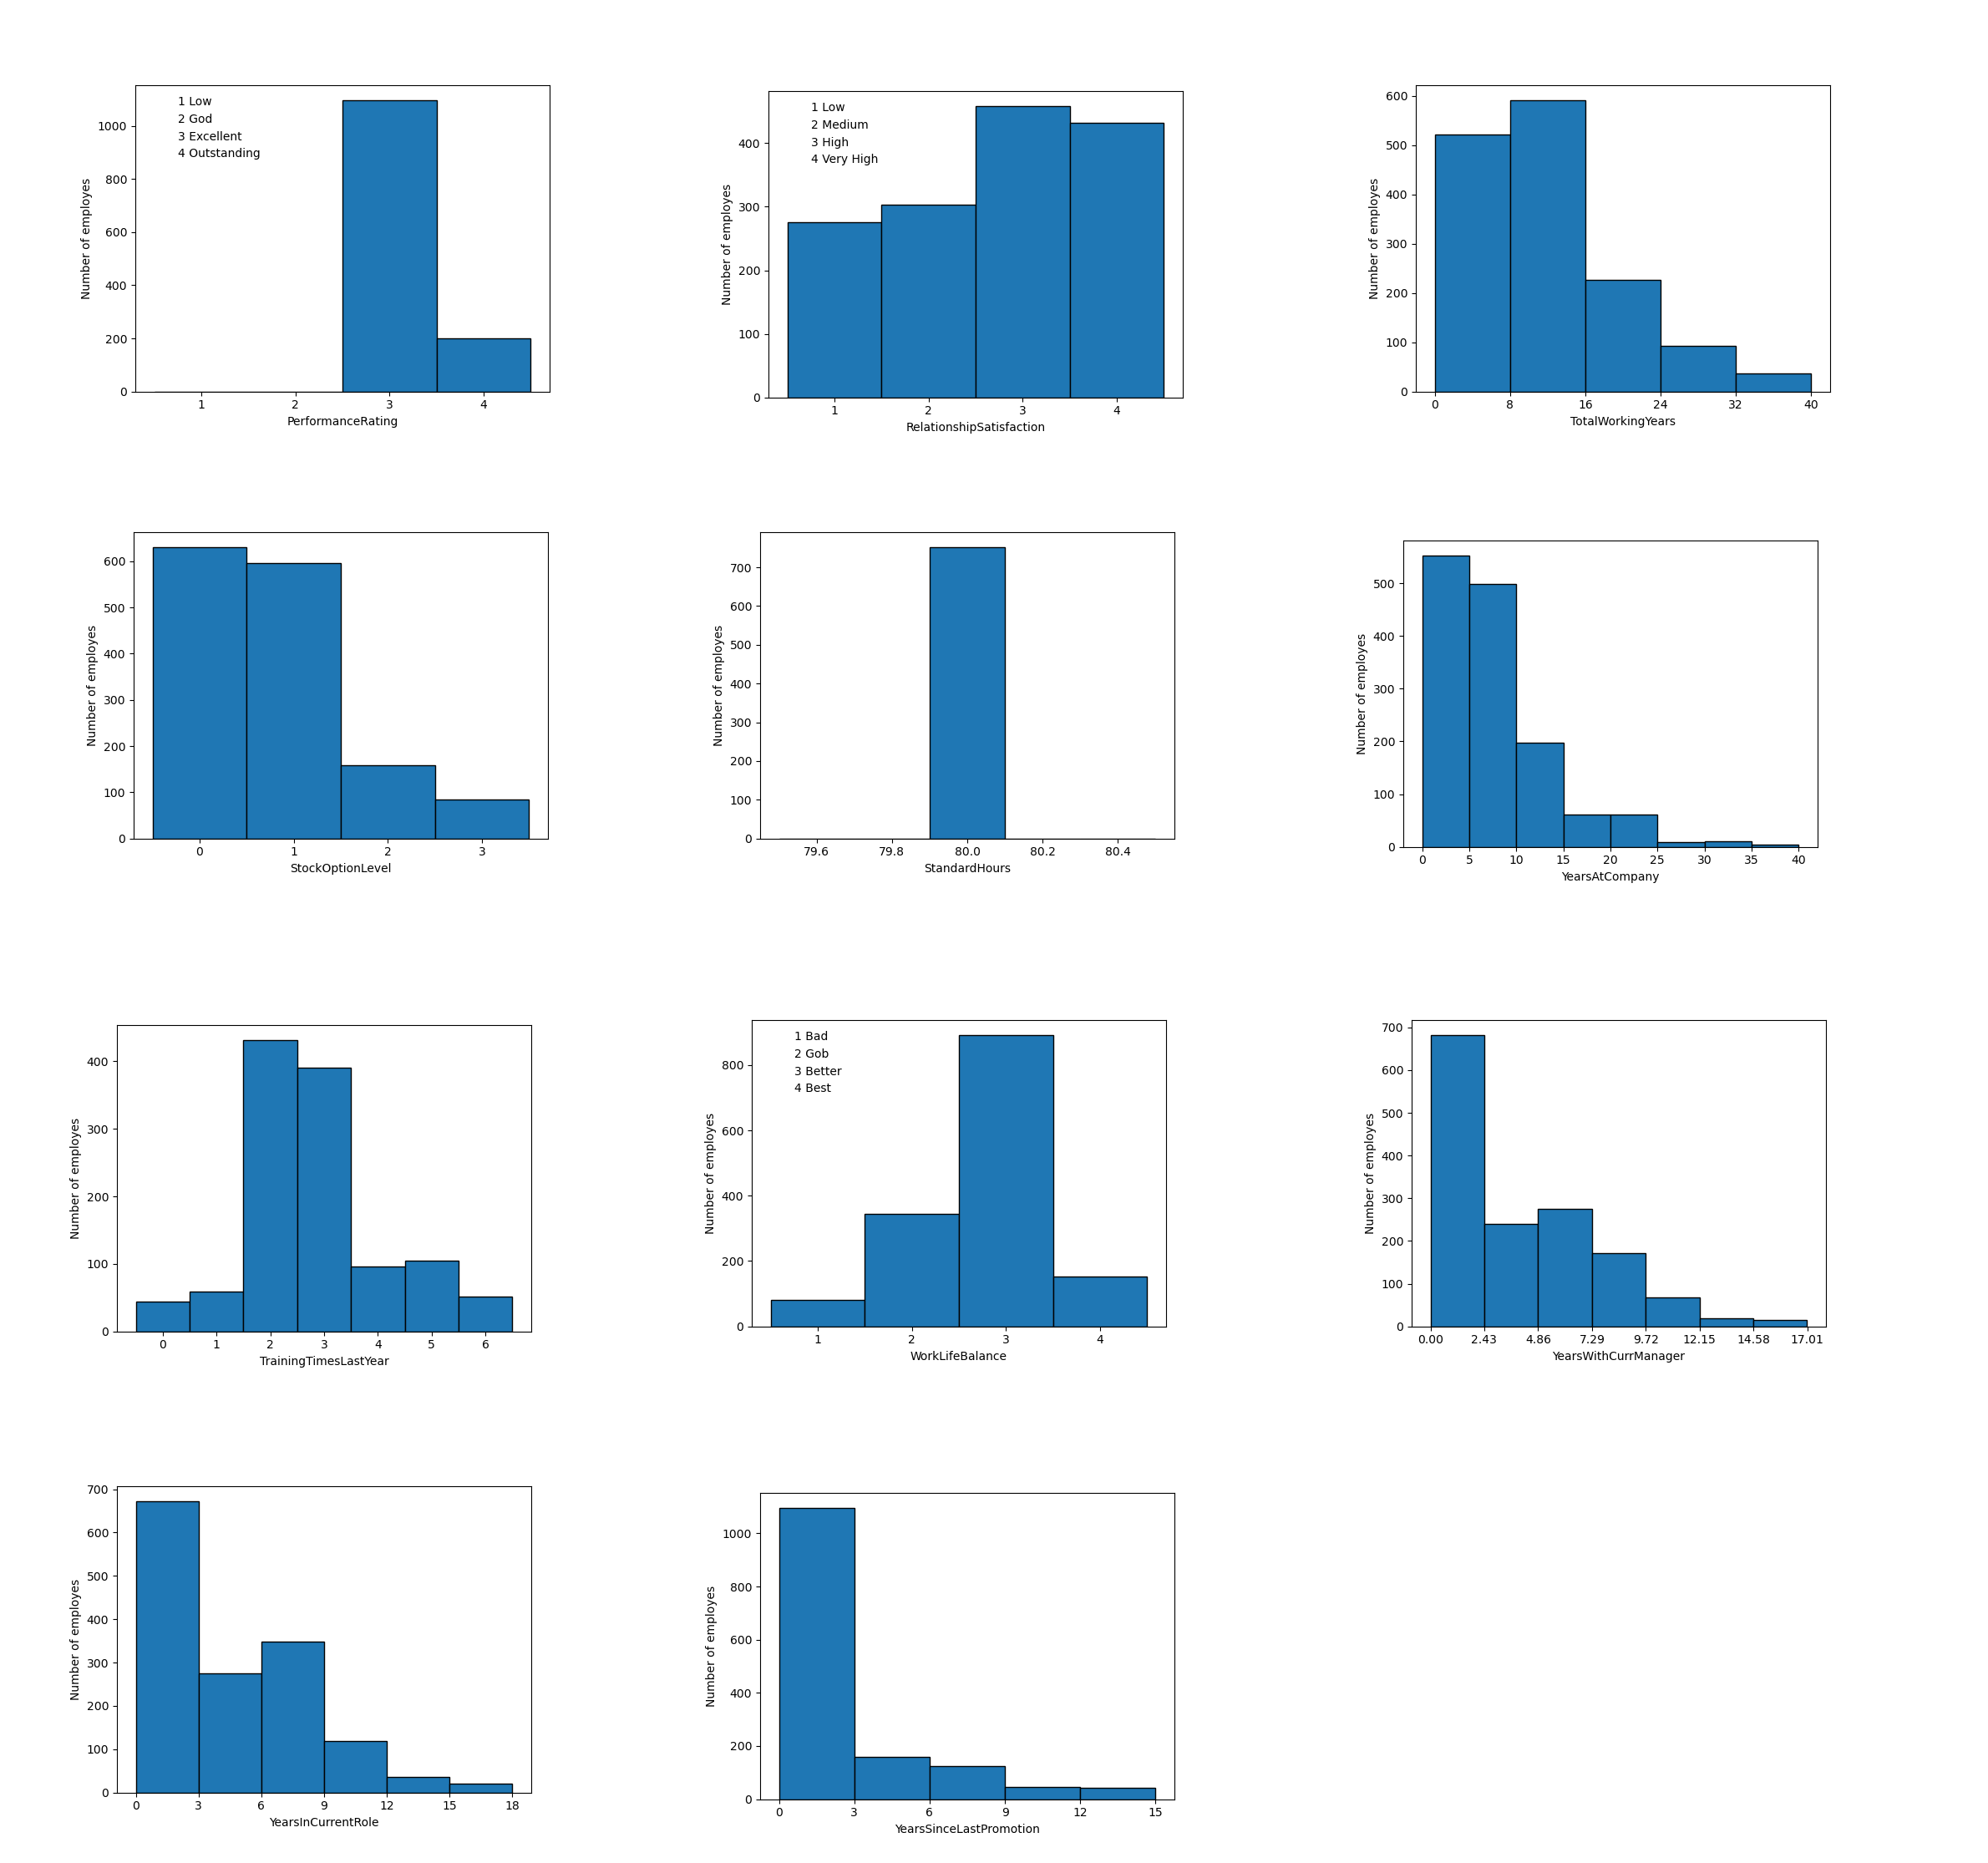
\includegraphics[scale=0.82,trim=0cm 0 0 0cm]{Istogrammi2.png}
\captionof{figure}{Istogrammi attributi numerici ed ordinali}
\end{center}

\subsection{Data Quality : Outliers e Missing values}
La qualità dei dati è fortemente influenzata negativamente dalla presenza di outliers e di missing values. Algoritmi di clustering e correlazioni fra gli attributi possono restituire risultati falsificati se non si gestiscono in maniera appropriata tali valori. 
Nel data frame utilizzato la loro presenza è evidente, infatti si ha che:

\begin{center}
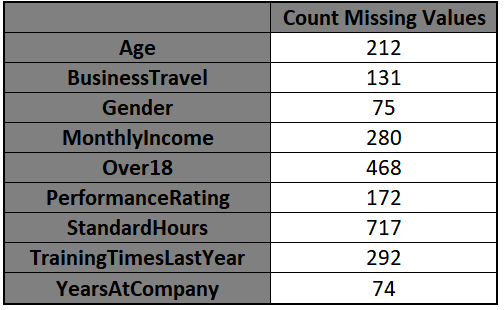
\includegraphics[scale=1.5]{missingvalues.png}
\captionof{figure}{Count dei missing values}
\end{center}
Gli attributi StandardHours ed Over18 presentano una qualità molto scarsa: nel primo circa la metà dei records sono mancanti e la restante parte ha un unico valore, mentre il secondo, oltre a contenere anch'esso una quantità significativa di missing values, non rappresenta in ogni caso un attributo di grande importanza, considerando che la stragrande maggioranza dei dipendenti di un'azienda sono maggiorenni. Per tali motivi, si è deciso di eliminare questi due attributi.

Per la determinazione degli outliers sono stati utilizzati sia test puramente statistici (Grubbs's test) che metodi di visualizzazione (Box Plot, Principal Component Analysis e scatter plot). Come è noto, per utilizzare approcci del primo tipo bisogna fare delle assunzioni sulla distribuzione sottostante dei valori esaminati. In particolare, il Grubbs's test, applicabile singolarmente agli attributi, richiede che i dati siano distribuiti normalmente, cosa non vera in questo caso. Di conseguenza, tale metodo è stato scartato. 
Il Principal Component Analysis, d'altro canto, è uno dei metodi maggiormente utilizzati nella ricerca di outliers in situazioni alto-dimensionali. Proiettando lo spazio n-dimensionale in uno spazio q-dimensionale ($q<n$), costruito tramite i vettori normalizzati della matrice di correlazione, si cerca di mantenere il più intatta possibile la varianza negli attributi. Nel caso in esame, la frazione di varianza conservata non risulta essere significativa (circa $0.4$), inficiando inevitabilmente i risultati ottenuti.
Anche la visualizzazione degli scatter plot confrontati con gli attributi categorici non ha evidenziato alcun punto identificabile come outlier.
L'unico metodo che ha avuto successo per la loro determinazione è stata la visualizzazione dei Box Plot per i singoli attributi. Si è proceduto quindi alla loro rimozione tramite eliminazione delle righe corrispondenti.

\section{Data Preparation}
In questa fase del lavoro ci si è posto l'obiettivo di trasformare e preparare il set di dati all'analisi successiva. I problemi precedentemente evidenziati sono stati qui risolti.\\

Come primo task sono stati gestiti i missing values.
L'attributo BusinessTravel presenta una frequenza di NaN pari al circa $9\%$, confrontabile con le frequenze degli altri valori . Siccome la granulosità dell'attributo ricopre in maniera completa lo spettro delle classi plausibilmente ad esso associabili, si è deciso di valutare se ci fosse dipendenza con gli altri attributi nel data frame. Per quanto riguarda quella con i numerici, sono stati utilizzati gli scatter plot, mentre per quelli nominali è stato eseguito il test di indipendenza del chi quadro. In entrambi i casi non si sono evinte dipendenze significative ($p value > 0.05$ sempre). Di conseguenza tale attributo è stato scartato.\\
Per quanto riguarda PerformanceRating, si è aggiunta una nuova classe 'MISSING', poiché si è notato che la granulosità dell'attributo in questo caso non ricopre tutto lo spettro plausibile. Si presuppone che i valori `MISSING' possano appartenere ad una classe di ordine inferiore ad `Excellent'.\\
Queste due considerazioni non sono applicabili all'attributo Gender per il quale si è scelto semplicemente di sostituire ai missing values valori estratti dalla distibuzione del campione.\\
Procedimento analogo è stato applicato a tutti gli attributi numerici che presentano valori mancanti, l'unica differenza è che in questo caso i valori sostitutivi sono le medie degli intervalli dei bins degli istogrammi.\\ %(che al mercato mio padre comprò, nda).\\
Come secondo task sono stati valutati gli outliers.\\
Il metodo di visualizzazione grafica dei Box Plot evidenzia la presenza di outliers solo in tre attributi numerici: TrainingTimeLastYear, TotalWorkingYears, YearsAtCompany
\begin{center}
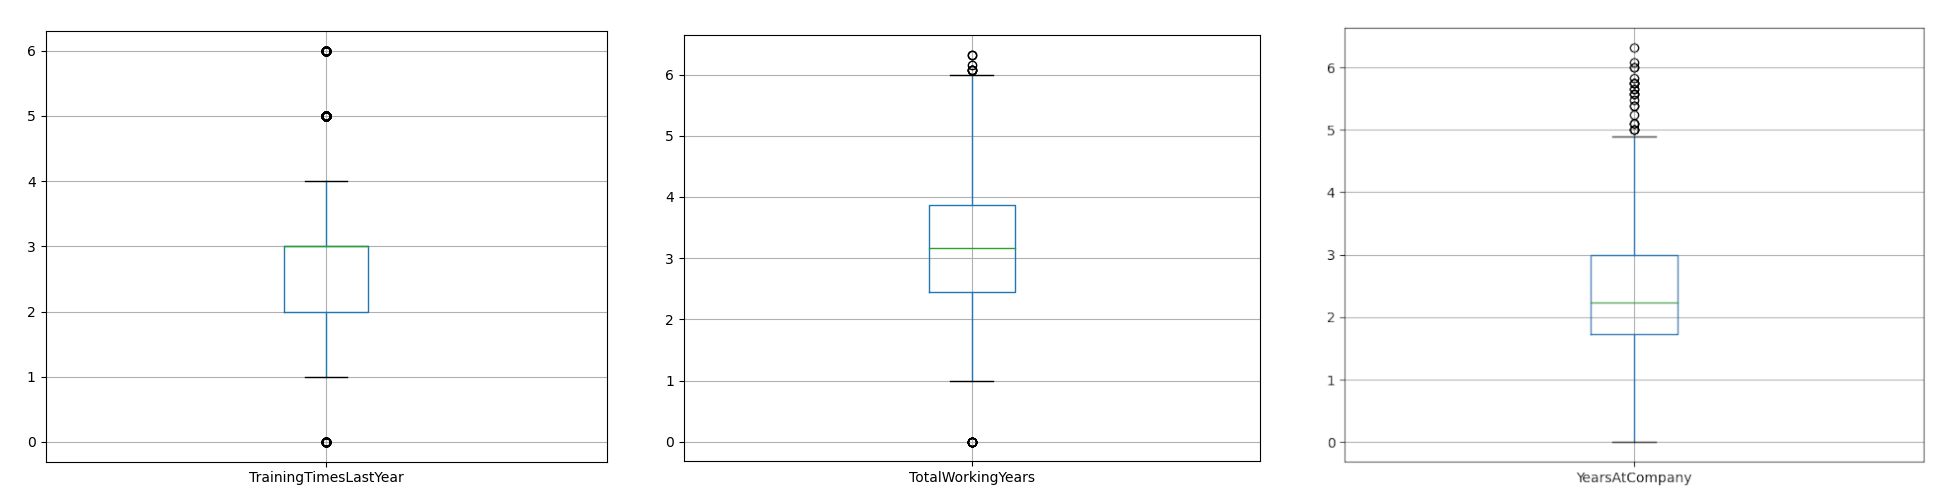
\includegraphics[scale=1]{boxplot.png}
\captionof{figure}{Box Plot degli attributi che presentano outliers}
\end{center}
 Il data frame dopo questa prima preparazione risulta contenere il $36\%$ di dati in meno rispetto a quello di partenza.\\
Funzioni di trasformazione sono state applicate ad attributi numerici con lo scopo di rimediare ad alcune caratteristiche delle loro distribuzioni, quali l'asimettrie e un valore spropositato della deviazione standar. In particolare è stata applicata la radice quadrata a DistanceFromHome (skew da 0.95 a 0.40), NumCompaniesWorked (skew da 1.03 a 0.03), PercentSalaryHike (skew da 0.82 a 0.65), TotalWorkingYears (skew da 1.12 a 0.18), YearsAtCompany (skew da 1.76 a 0.43), YearsInCurrentRole(skew da 0.92 a $-$0.25), YearsSinceLastPromotion (skew da 1.98 a 0.74) e YearsWithCurrManager (skew da 0.83 a $-$0.25); invece a MonthlyIncome è stato applicato il logaritmo naturale (varianza da 4710 a 0.67) . Di seguito sono riportate alcune distribuzioni delle variabili trasformate.\\

\begin{center}
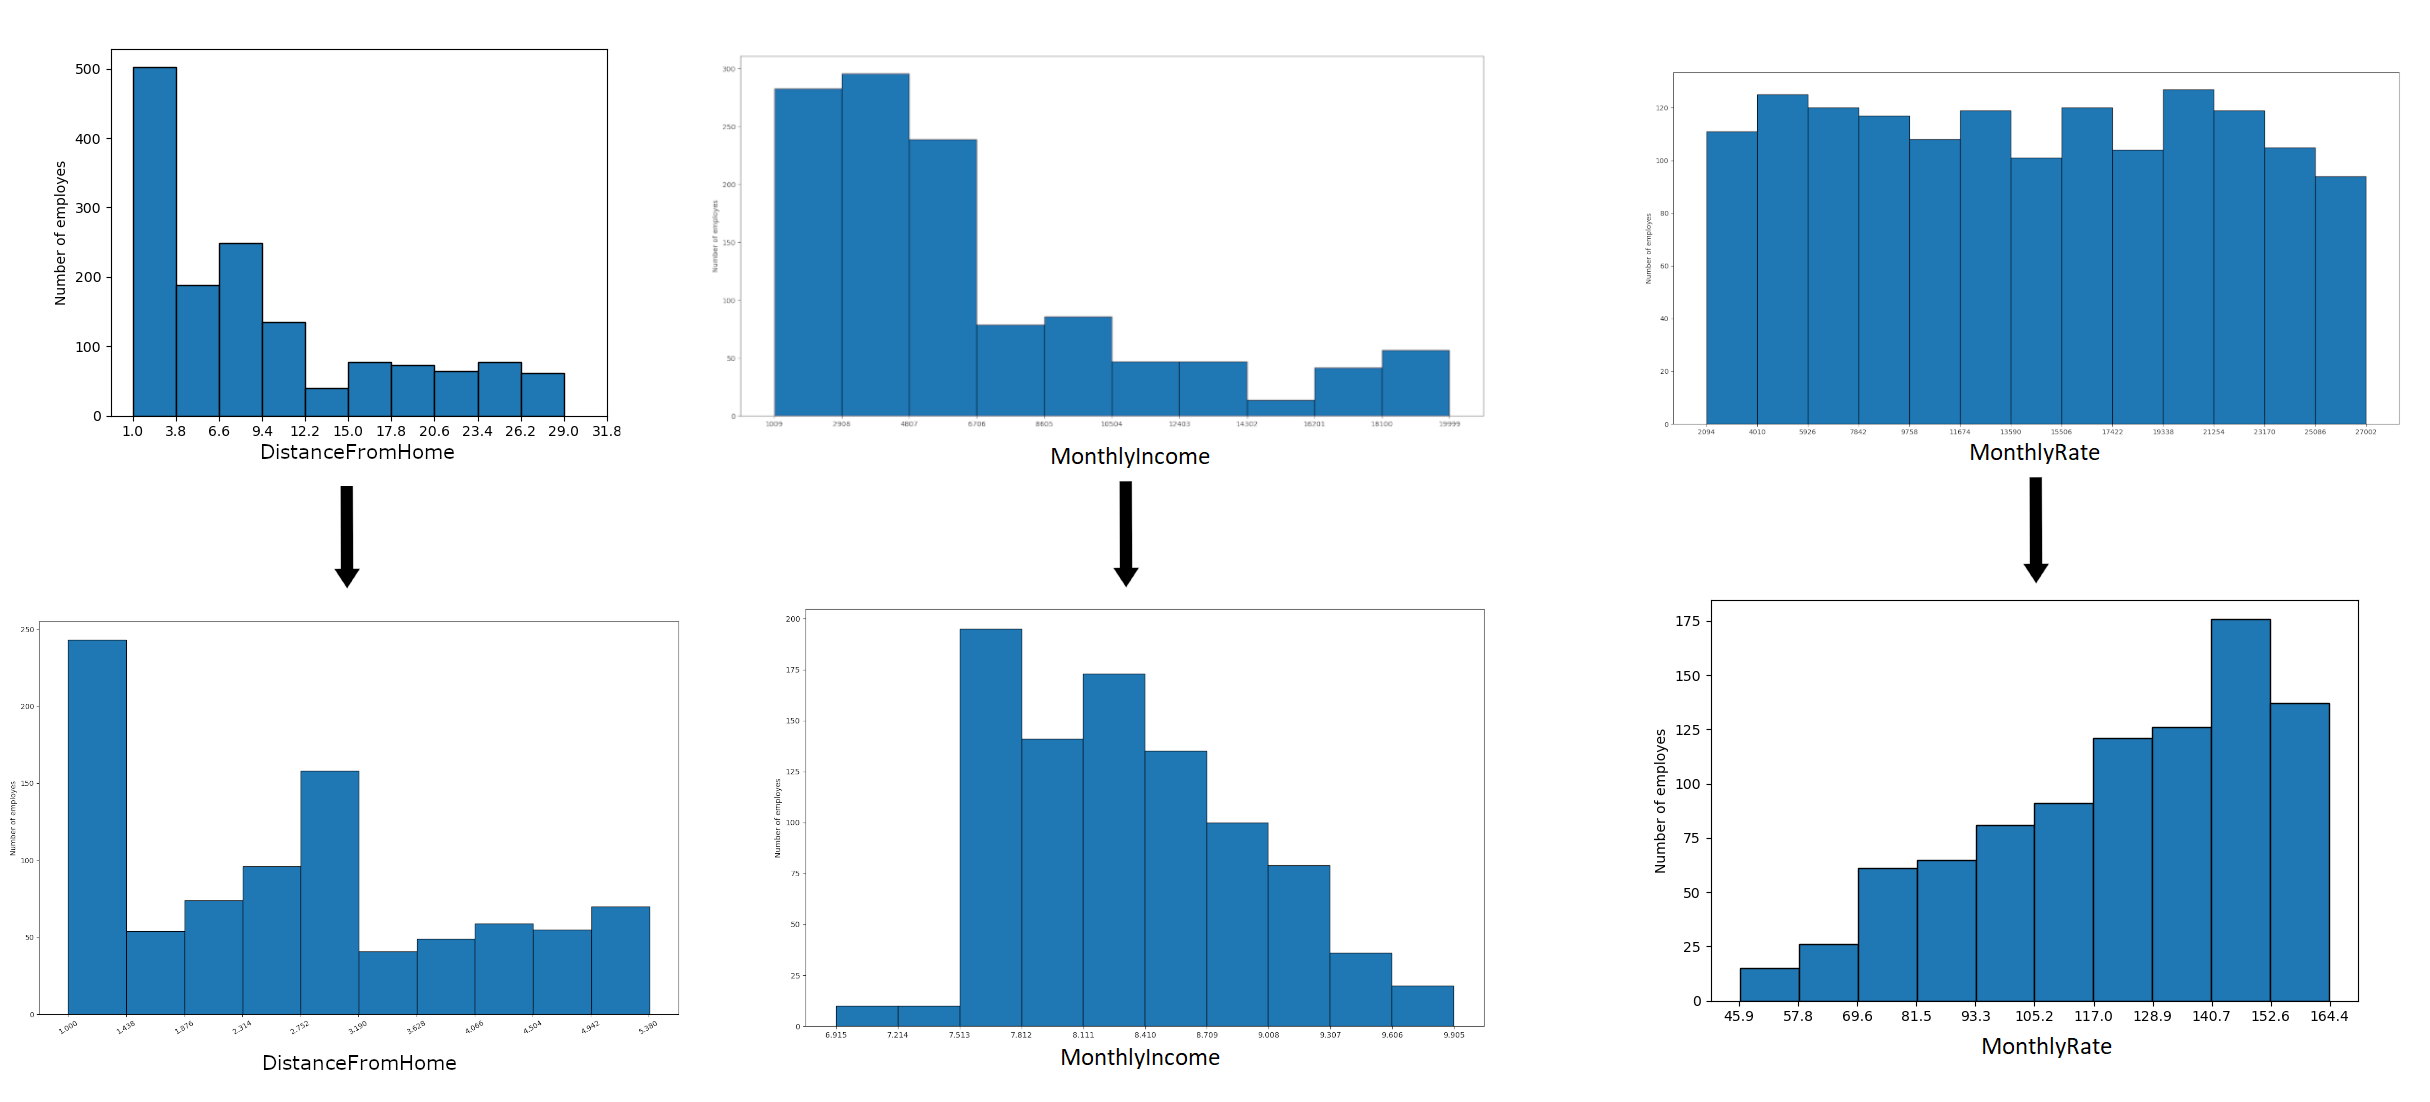
\includegraphics[scale=0.35]{trasformer.png}
\captionof{figure}{Distribuzione di alcune variabili trasformate}
\end{center}

Come terzo task sono stati eliminati ed aggiunti nuovi attributi.\\
In luogo di TotalWorkingYears e YearsAtCompany si è scelto di introdurre il loro rapporto, denominato FractionAtCompany che rappresenta la frazione di anni lavorativi del singolo dipendente nell'azienda. Tramite l'introduzione di tale attributo è stato possibile notare l'inconsistenza di alcuni records per cui tale rapporto risultava essere maggiore di 1. Tali valori sono stati eliminati. Analogamente si è proceduto per MonthlyIncome e MonthlyRate sostituiti da RateIncome, indice di quanto l'azienda spende per un impiegato in rapporto al suo stipendio. Anche in questo caso sono stati eliminati i valori inconsistenti.\\ 
DailyRate e HourlyRate contengono la stessa informazione di MonthlyRate, quindi sono stati eliminati.\\
Inoltre, YearsInCurrentRole, YearInCurrManager e YearsSinceLastPromotion sono caratterizzati da una correlazione significativa e quindi si è deciso di mantenere solamente YearsInCurrentRole nell'analisi a seguire.\\
Infine è stata calcolata la matrice di correlazione lineare fra gli attributi numerici e i valori del $p $ $value$  ottenuti tramite test del chi quadro per l'interdipendenza fra gli attributi categorici.\\
Si può notare come il $p$ $ value$ per la maggioranza dei casi è maggiore di $0.05$, valore scelto come soglia; questo significa che l'ipotesi nulla (non c'è relazione tra i due attributi) non può essere scartata. Nell'altra situazione invece l'evidenza empirica è fortemente contraria all'ipotesi nulla, ciò significa che la presenza di una dipendenza tra gli attributi è statisticamente plausibile, come ad esempio avviene tra Attrition (quanto un impiegato è "logorato") e MaritialStatus (condizione sentimentale dell'impiegato).\\
Per gli attributi numerici, in seguito alle trasformazione effettuate, non sono presenti corelazioni significative.

\begin{center}
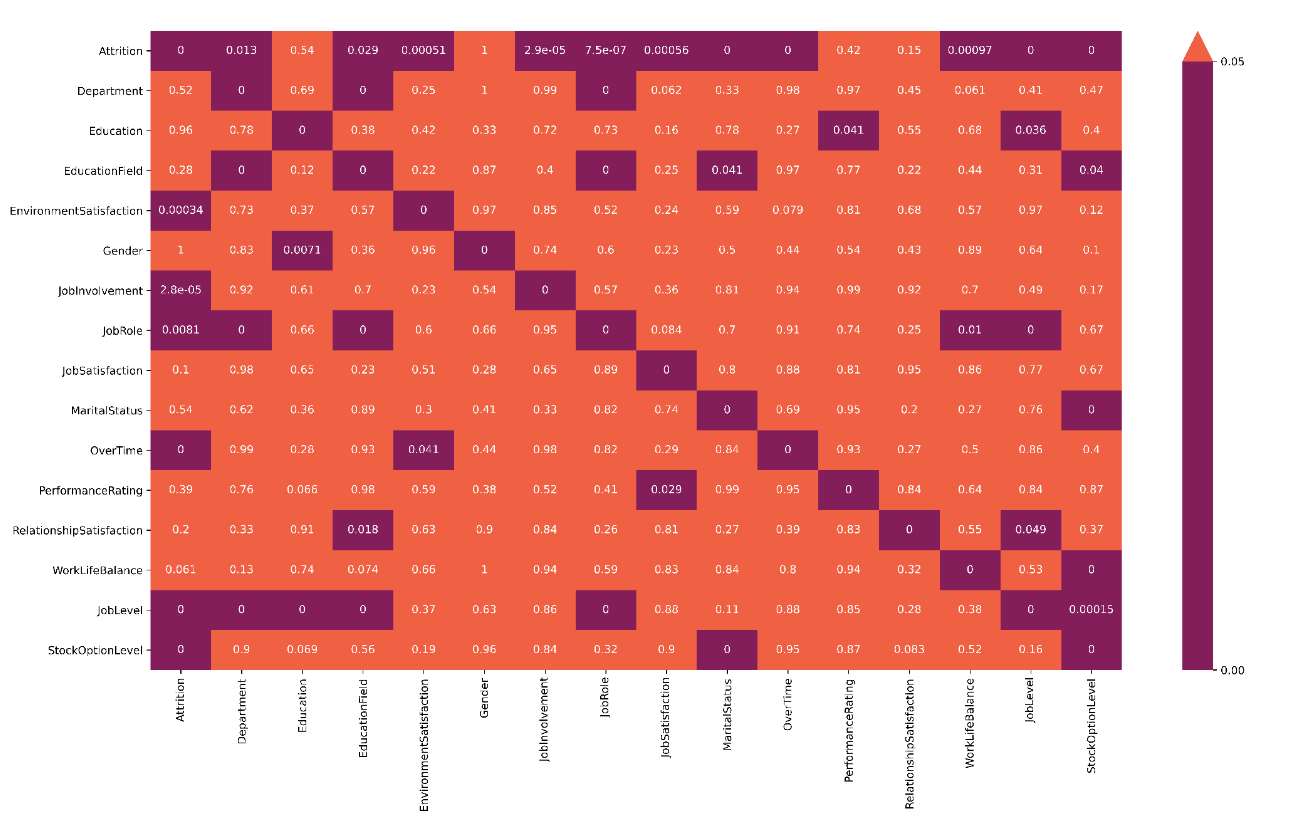
\includegraphics[scale=1.2]{mccat.png}
\captionof{figure}{Matrice dei $p$ $value$ per gli attributi categorici}
\end{center}

\begin{center}
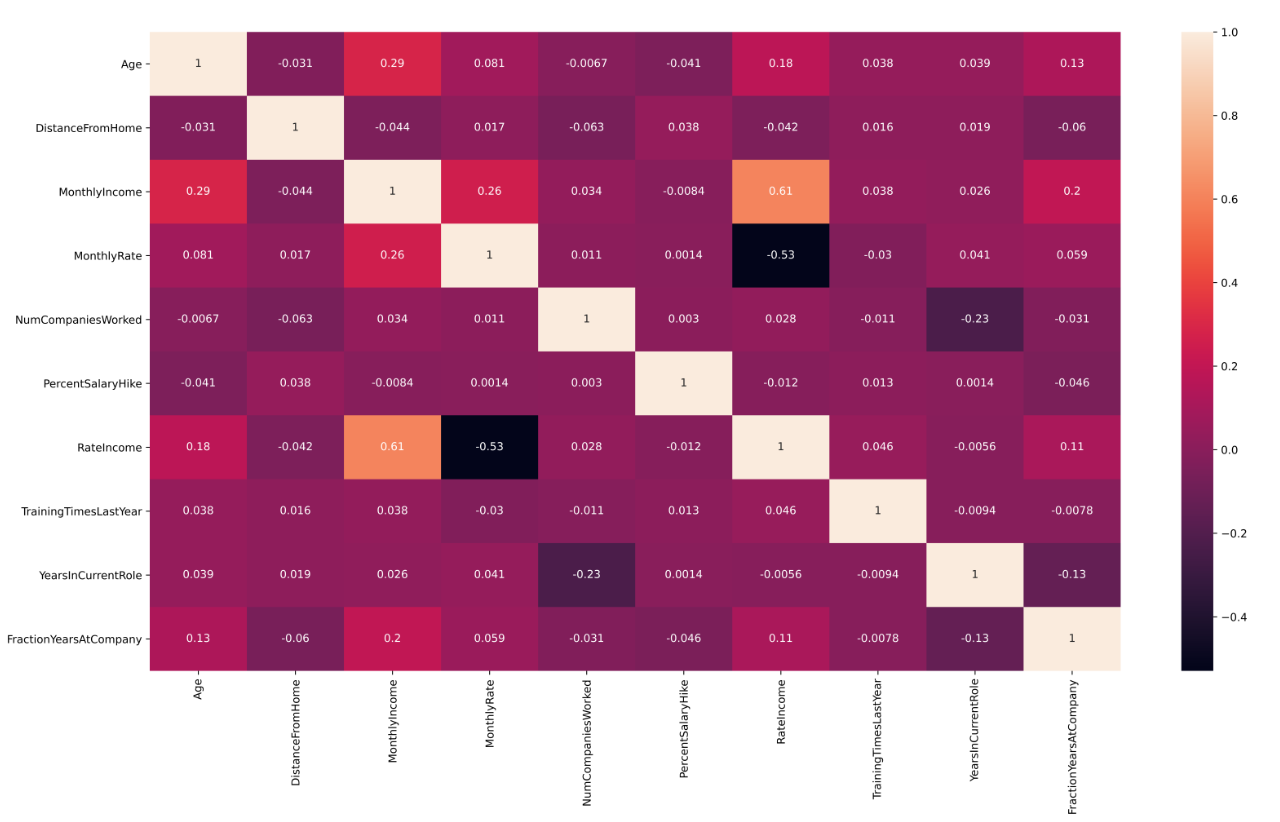
\includegraphics[scale=1.2]{macnum.png}
\captionof{figure}{Matrice di correlazione per gli attributi numerici}
\end{center}

\section{Clustering}
Preparato il data frame si è proceduto all'analisi degli algoritmi di clustering: K-Means, DB Scan e Hierarchical. La dimensionalità del data frame ($10$) è stata considerata troppo elevata per ottenere risultati consistenti, quindi sono stati indagati sottoinsiemi 3-5 dimensionali alla ricerca un qualche tipo di clusterizzazione. 
Come metrica è stata usata la distanza euclidea, i dati sono stati inoltre normalizzati tra $0$ e $1$.\\
Si vuole precisare che per la visualizzazione dei clusters ottenuti tramite K-Means e DB Scan è stato utilizzato uno spazio tridimensionale poichè, soprattutto nel primo caso, una visualizzazione bidimensionale portava ad un mixing eccesivo dei clusters stessi.

\subsection{K-Means}
Per quanto riguarda il K-Means i sottoinsiemi che hanno mostrato i risultati migliori sono:\\

\begin{enumerate}
\item PercentSalaryHike, FractionYearsAtCompany, YearsInCurrentRole, RateIncome, NumCompaniesWorked
\item DistanceFromHome, FractionYearsAtCompany, RateIncome, YearsInCurrentRole, TrainingTimesLastYear
\item DistanceFromHome, RateIncome, Age, FractionYearsAtCompany
\item DistanceFromHome, FractionYearsAtCompany, TrainingTimesLastYear, PercentSalaryHike, YearsInCurrentRole
\end{enumerate}


\begin{center}
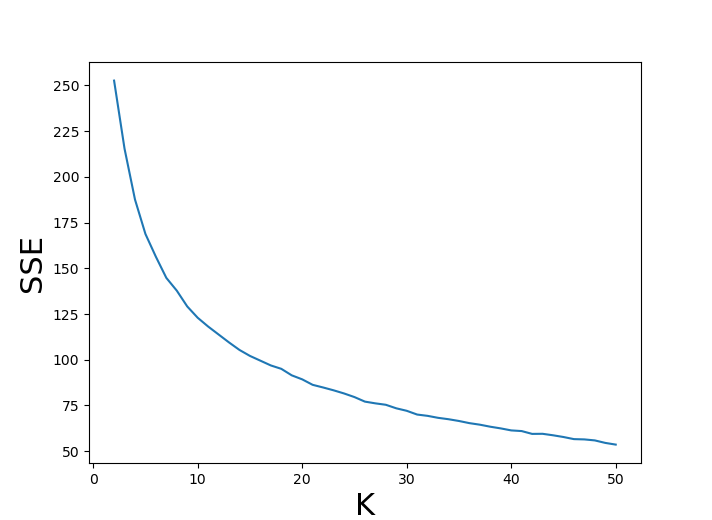
\includegraphics[scale=0.6]{SSEsub1.png}
\captionof{figure}{SSE in funzione di $K$}
\end{center}

La scelta del numero di cluster $K$ è stata presa osservando l'andamento del SSE in funzione di $K$ (Figura $12$), simile in tutti e quattro i casi esaminati; con lo scopo di aver un buon compromesso fra i due l'algoritmo è stato eseguito per $K$ uguale a 3, 4 e 5. Dai risultati ottenuti si evince che, sebbene con $K=5$ il valore delle SSE è minore rispetto agli altri due casi, non si apprezzano cluster evidenti: ve ne sono sempre due eccessivamente mescolati. Con $K=3$ la divisione fra i clusters è sicuramente ben evidente ma, con $K=4$, si ottengono comunque buoni risultati con il vantaggio di un SSE minore. \\
Nei seguenti grafici sono mostrati i risultati ottenuti e per redendere più chiara la posizione dei centroidi, sono riportate anche le loro cordinate organizzate in parallelo per ciascun sottoinsieme usato.

\begin{figure}[H]
\begin{minipage}[b]{0.47\textwidth}
\centering
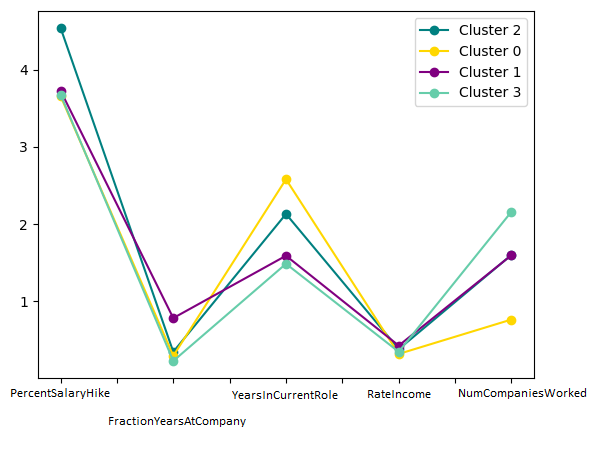
\includegraphics[width=\textwidth]{parallelsub1.png}
\caption{Parallel coordinates dei centroidi}
\label{etichetta1}
\end{minipage}
\hfill
\begin{minipage}[b]{0.55\textwidth}
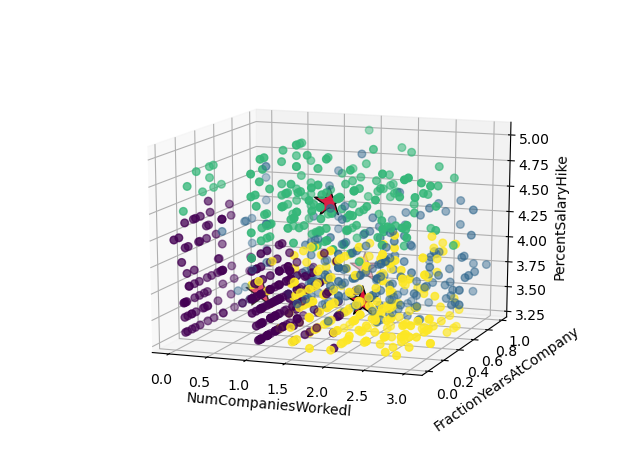
\includegraphics[scale=0.6]{numcompan_Fraction_percentCENTROIDI.png}
\caption{Cluster sottoinsime 1: SSE$=187$; silhouette$=0.18$}
\label{etichetta2}
\end{minipage}
\end{figure}

\begin{figure}[H]
\begin{minipage}[b]{0.47\textwidth}
\centering
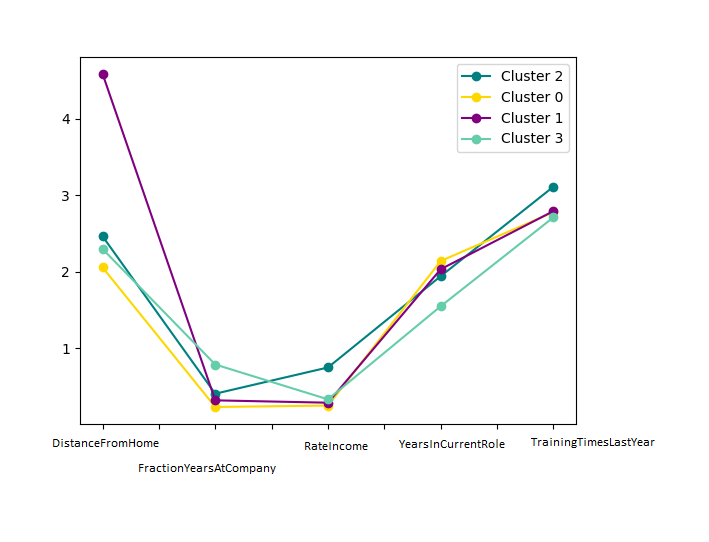
\includegraphics[width=\textwidth]{par_cor2.png}
\caption{Parallel coordinates dei centroidi}
\label{etichetta1}
\end{minipage}
\hfill
\begin{minipage}[b]{0.55\textwidth}
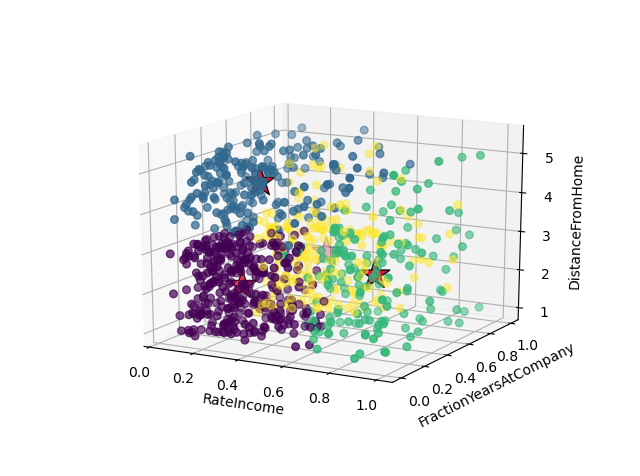
\includegraphics[scale=0.6]{rate_fraction_distance2.png}
\caption{Cluster sottoinsime 2: SSE$=177$; silhouette$=0.21$}
\label{etichetta2}
\end{minipage}
\end{figure}

\begin{figure}[H]
\begin{minipage}[b]{0.47\textwidth}
\centering
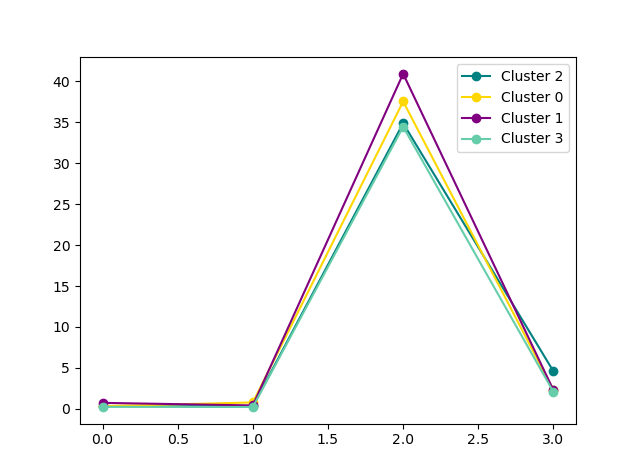
\includegraphics[width=\textwidth]{par_cor_centroid8.png}
\caption{Parallel coordinates dei centroidi}
\label{etichetta1}
\end{minipage}
\hfill
\begin{minipage}[b]{0.55\textwidth}
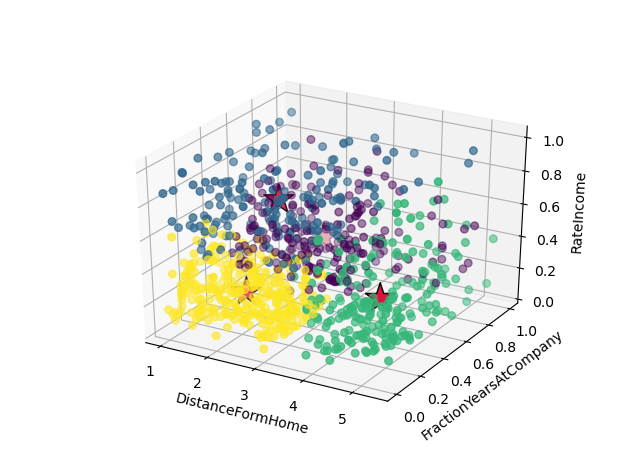
\includegraphics[scale=0.6]{rate_frac_dist8.png}
\caption{Cluster sottoinsime 3: SSE$=129$; silhouette$=0.25$}
\label{etichetta2}
\end{minipage}
\end{figure}

\begin{figure}[H]
\begin{minipage}[b]{0.47\textwidth}
\centering
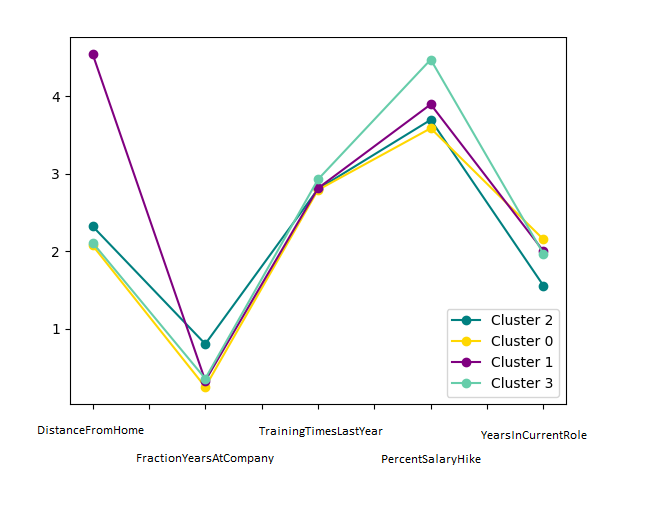
\includegraphics[width=\textwidth]{parr cor frac6.png}
\caption{Parallel coordinates dei centroidi}
\label{etichetta1}
\end{minipage}
\hfill
\begin{minipage}[b]{0.55\textwidth}
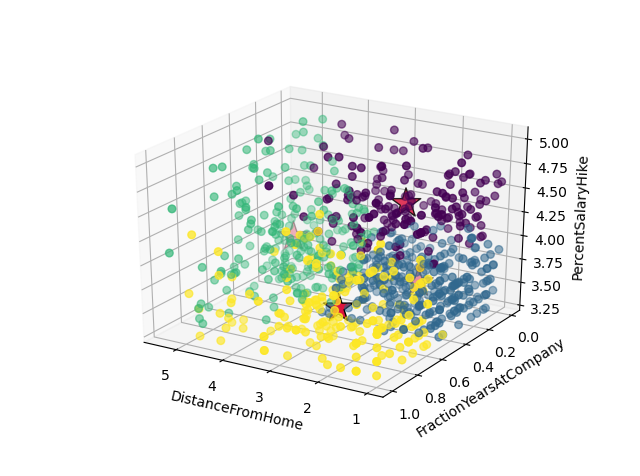
\includegraphics[scale=0.6]{FractionYear_Distance_Percent_CENTROIDI6.png}
\caption{Cluster sottoinsime 4: SSE$=182$; silhouette$=0.20$}
\label{etichetta2}
\end{minipage}
\end{figure}

Dalla divisione in cluster è possibile classificare gli impiegati in base ad alcune caratteristiche comuni.
Ad esempio il cluster giallo nella Figura $13$  esprime l'irrilevanza dell'esperienza lavorativa al di fuori dell'azienda relativamente all'aumento di stipendio. Infatti chi è stato assunto da poco (rispetto alla vita lavorativa), sebbene abbia maturato esperienza in altre aziende, ha un percent salary hike basso.
D'altro canto, al cluster viola è plausibile associare i lavoratori la cui esperienza è costituita quasi esclusivamente da ruoli indipendenti da compagnie. Anche in questo caso, il percent salary hike è relativamente basso.
Il cluster blu può essere considerato il gruppo di lavoratori la cui esperienza non è stata influenzata da altri impieghi nel passato. Infatti si nota che in questo caso l'aumento percentuale dello stipendio è indipendente dal numero di compagnie precedenti.
Infine il cluster verde può essere visto come il gruppo di persone che hanno acquisito competenze utili all'azienda (ciò è evidente dalla percentuale di aumento di stipendio molto alta rispetto a tutti gli altri gruppi) in altri ambienti.\\
La classificazione fatta non è certamente da considerarsi assoluta, poiché dai valori della silhouette non elevati, si capisce che la distinzione tra i cluster non è netta: mescolamenti tra di essi sono molto plausibili.
Ragionamenti simili possono essere applicati agli altri grafici.

\subsubsection{Validazione}
Per quanto riguarda la validazione dei cluster ottenuti, si è valutata la distribuzione dell'SSE e della silhouette generati dal K-Means su un numero $N=500$ di set di dati random estratti dallo stesso dominio degli attributi usati. La clusterizzazione è quindi ritenuta non random se l'SSE e la silhouette sono al di fuori di quattro deviazioni standard dal valor medio, ciò assicura che i dati ottenuti sono esterni al $99.994\%$  delle relative distribuzioni.
Dalle immagini seguenti si evince che tutti i valori ottenuti sono compatibili con una clusterizzazione non random.

\begin{figure}[H]
\begin{minipage}[b]{0.45\textwidth}
\centering
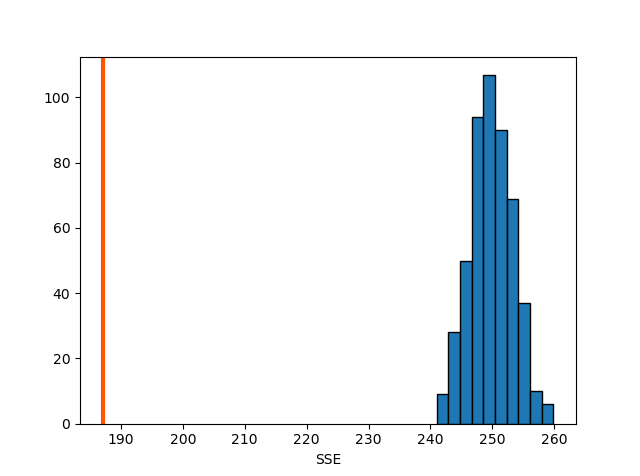
\includegraphics[width=\textwidth]{RandomSSE_1.png}
\caption{Distribuzione dell'SSE su 500 set di dati random per il sottoinsieme 1. Media: 250; Deviazione Standard: 3. La linea arancione rappresenta l'SSE sui dati reali.  }
\label{etichetta1}
\end{minipage}
\hfill
\begin{minipage}[b]{0.45\textwidth}
\centering
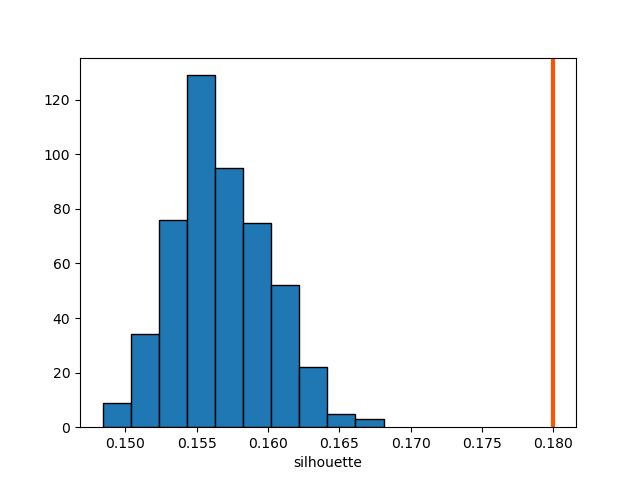
\includegraphics[width=\textwidth]{RandomSilhouette_1.png}
\caption{Distribuzione della silhouette su 500 set di dati random per il sottoinsieme 1. Media: 0.156; Deviazione Standard: 0.003. La linea arancione rappresenta la silhouette sui dati reali.}
\label{etichetta2}
\end{minipage}
% \end{figure}
% \begin{figure}[H]
% \begin{minipage}[b]{0.45\textwidth}
% \centering
% 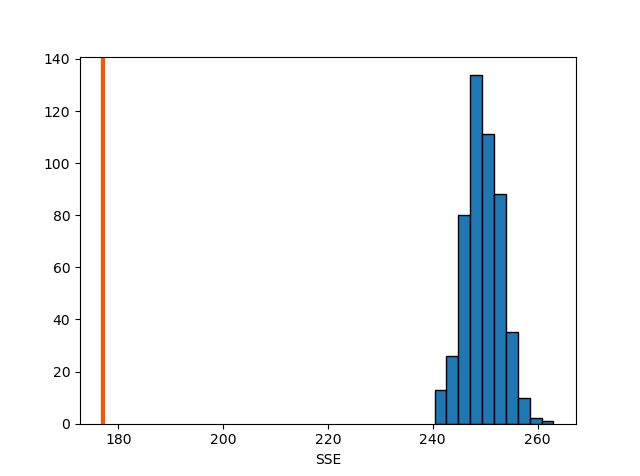
\includegraphics[width=\textwidth]{RandomSSE_2.png}
% \caption{Distribuzione dell'SSE su 500 set di dati random per il sottoinsieme 2. Media: 250; Deviazione Standard: 3. La linea arancione rappresenta l'SSE sui dati reali.}
% \label{etichetta1}
% \end{minipage}
% \hfill
% \begin{minipage}[b]{0.45\textwidth}
% \centering
% 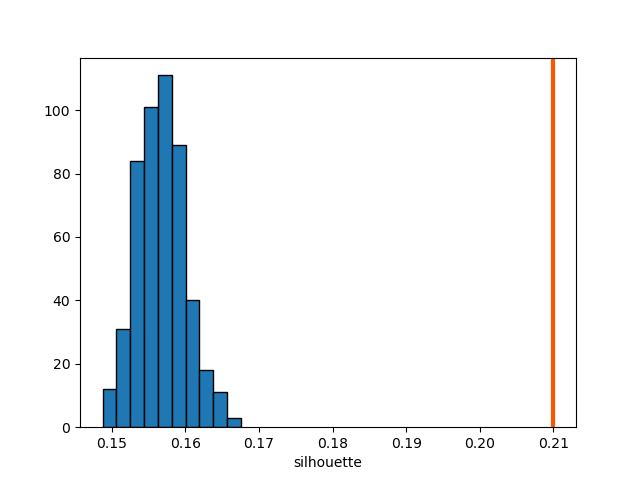
\includegraphics[width=\textwidth]{RandomSilhouette_2.png}
% \caption{Distribuzione della silhouette su 500 set di dati random per il sottoinsieme 2. Media: 0.156; Deviazione Standard: 0.003. La linea arancione rappresenta la silhouette sui dati reali. }
% \label{etichetta2}
% \end{minipage}
% \begin{minipage}[b]{0.45\textwidth}
% \centering
% 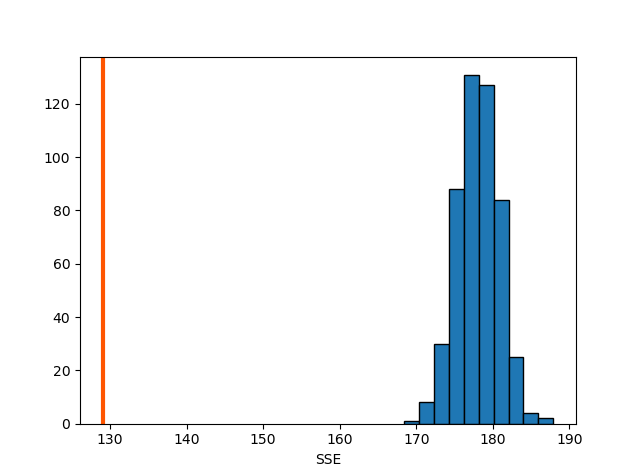
\includegraphics[width=\textwidth]{RandomSSE_3.png}
% \caption{Distribuzione dell'SSE su 500 set di dati random per il sottoinsieme 3. Media: 178; Deviazione Standard: 3. La linea arancione rappresenta l'SSE sui dati reali.  }
% \label{etichetta1}
% \end{minipage}
% \hfill
% \begin{minipage}[b]{0.45\textwidth}
% \centering
% 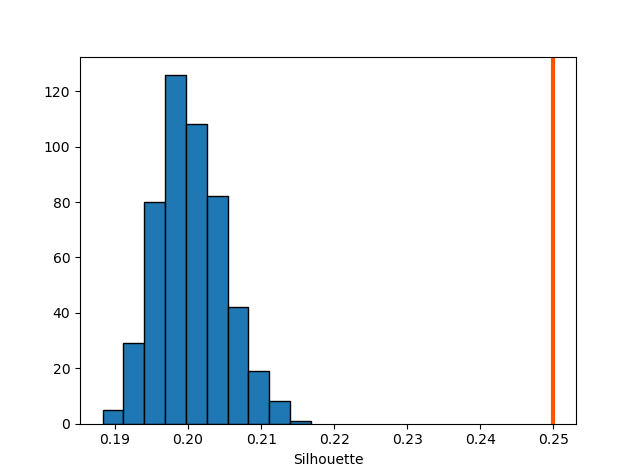
\includegraphics[width=\textwidth]{RandomSilhouette_3.png}
% \caption{Distribuzione della silhouette su 500 set di dati random per il sottoinsieme 3. Media: 0.200; Deviazione Standard: 0.004. La linea arancione rappresenta la silhouette sui dati reali.}
% \label{etichetta2}
% \end{minipage}
% \end{figure}
% \begin{figure}[H]
% \begin{minipage}[b]{0.45\textwidth}
% \centering
% 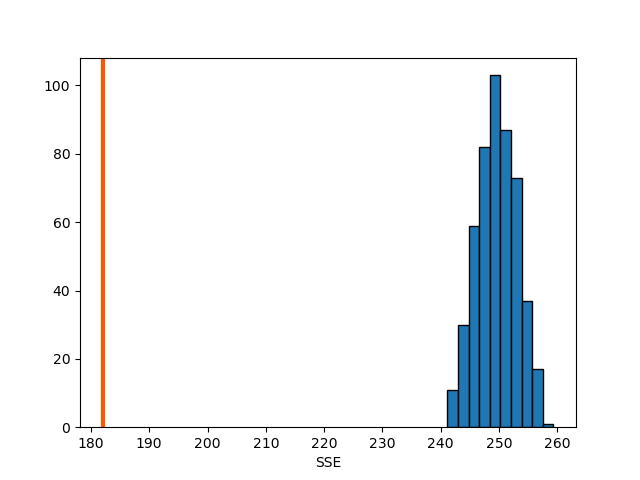
\includegraphics[width=\textwidth]{RandomSSE_4.png}
% \caption{Distribuzione dell'SSE su 500 set di dati random per il sottoinsieme 4. Media: 250; Deviazione Standard: 3. La linea arancione rappresenta l'SSE sui dati reali.}
% \label{etichetta1}
% \end{minipage}
% \hfill
% \begin{minipage}[b]{0.45\textwidth}
% \centering
% \includegraphics[width=\textwidth]{RandomSilhouette_4.png}
% \caption{Distribuzione della silhouette su 500 set di dati random per il sottoinsieme 4. Media: 0.156; Deviazione Standard: 0.003. La linea arancione rappresenta la silhouette sui dati reali. }
% \label{etichetta2}
% \end{minipage}
\end{figure}



\subsection{DB-Scan}
Per quanto riguarda il DB-Scan i sottoinsiemi che sono stati utilizzati :\\
\begin{enumerate}
\item PercentSalaryHike, FractionYearsAtCompany, YearsInCurrentRole, RateIncome
\item PercentSalaryHike, FractionYearsAtCompany, RateIncome, YearsInCurrentRole, NumCompaniesWorked
\item DistanceFromHome, FractionYearsAtCompany, RateIncome, YearsInCurrentRole, TrainingTimesLastYear
\end{enumerate}

La sensibilità dell'algoritmo alla scelta dei parametri è molto più elevata rispetto al K-Means. L'approccio utilizzato è stato quello di far variare il numero di min samples tra $5$ e $20$ e, attraverso il grafico dell'elbow curve, è stato scelto il valore di $eps$ in prossimità del gomito. Successivamente è stato fatto variare il valore di $eps$ su una scala molto fine in un suo intorno.

\begin{figure}[H]
\begin{minipage}[b]{0.45\textwidth}
\centering
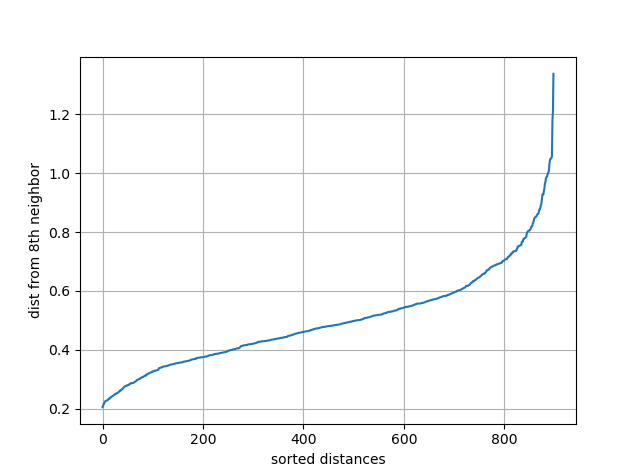
\includegraphics[width=\textwidth]{Figure_1.png}
\caption{Sottoinsieme 1. Elbow curve con min samples =  8 }
\label{etichetta1}
\end{minipage}
\hfill
\begin{minipage}[b]{0.45\textwidth}
\centering
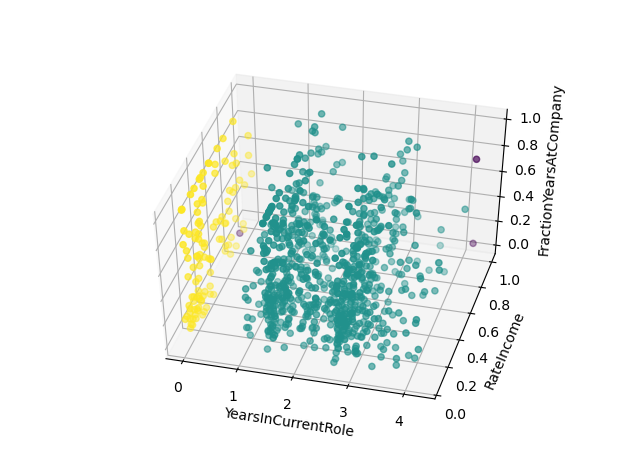
\includegraphics[width=\textwidth]{Figure_24.png}
\caption{Sottoinsieme 1. eps = 0.750 , silhoutte = 0.26 }
\label{etichetta2}
\end{minipage}
\end{figure}


\begin{figure}[H]
\begin{minipage}[b]{0.45\textwidth}
\centering
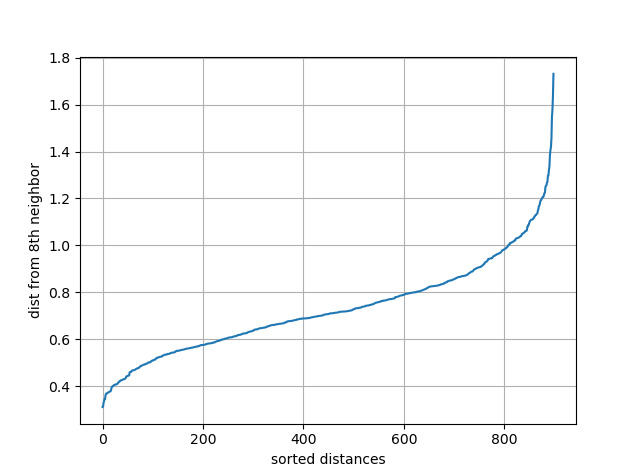
\includegraphics[width=\textwidth]{2.png}
\caption{Sottoinsieme 2. Elbow curve con min samples =  8}
\label{etichetta1}
\centering
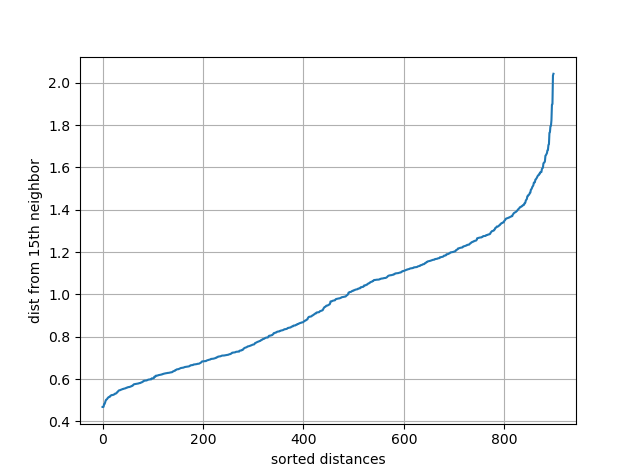
\includegraphics[width=\textwidth]{5 (1).png}
\caption{Sottoinsieme 3. Elbow curve con min samples =  15}
\label{etichetta1}
\end{minipage}
\hfill
\begin{minipage}[b]{0.45\textwidth}
\centering
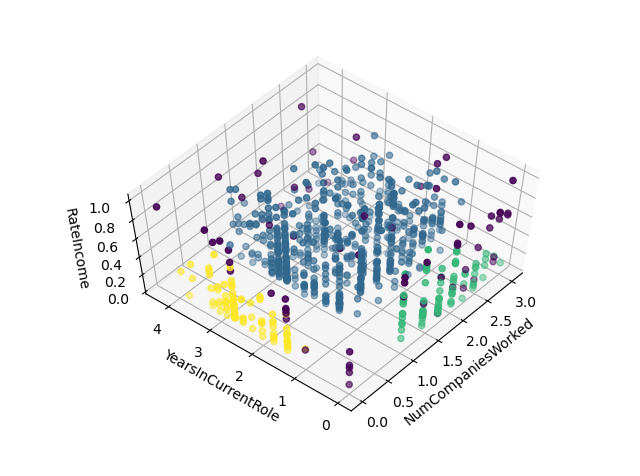
\includegraphics[width=\textwidth]{22.png}
\caption{Sottoinsieme 2. eps = 0.950, silhoutte = 0.12 }
\label{etichetta2}
\centering
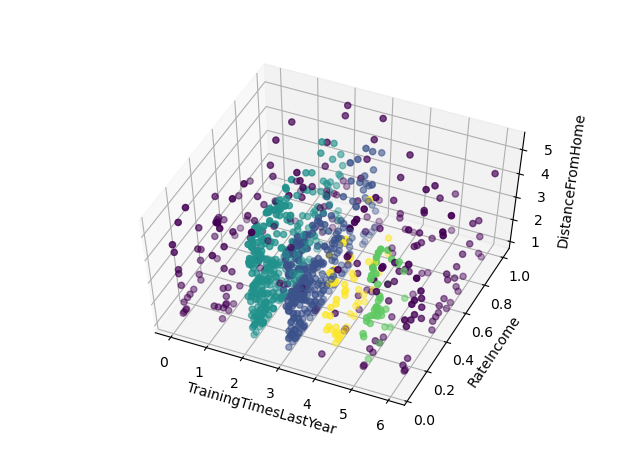
\includegraphics[width=\textwidth]{5 (2).png}
\caption{Sottoinsieme 3. eps = 1.20, silhoutte = 0.02}
\label{etichetta2}
\end{minipage}
\end{figure}

Come si può notare dai grafici l'algoritmo è riuscito ad evidenziare un diverso numero di cluster ed un certo numero di noise points (punti viola). Questo è essenzialmente dovuto alla distribuzione dei valori nello spazio tridimensionale: essi formano infatti delle slices molto dense a valori fissati di uno dei tre attributi, come si può ad esempio osservare nella Figura 33. In questo caso inoltre si nota che il valore della silhoutte è praticamente nullo e ciò implica che la divisione ottenuta è totalmente inconsistente. Per tali motivi non è stato possibile associare ai cluster alcun significato.

\subsubsection{Validazione}
La validazione è stata eseguita anche in questo caso tramite la costruzione di $N_1=35000$ e $N_2=10^3$ distribuzioni random su cui si è valutata la silhouette. La clusterizzazione è stata considerata non random se il valore ottenuto della silhouette è al di fuori di quattro deviazioni standard dal valor medio, quindi esterno al $99.994\%$ della distribuzione.
Come si può notare dal secondo grafico i risultati otteneuti sono da scartare.
\begin{figure}[H]
\begin{minipage}[b]{0.45\textwidth}
\centering
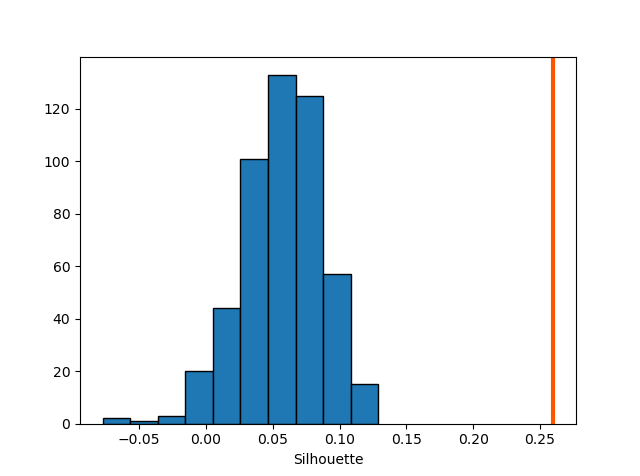
\includegraphics[width=\textwidth]{RandomSilhouetteDBSCAN_1.png}
\caption{Distribuzione della silhouette su $N_1$ per il sottoinsieme 1. Media: 0.06; Deviazione Standard: 0.03. La linea arancione rappresenta la silhouette sui dati reali.  }
\label{etichetta1}
\end{minipage}
\hfill
\begin{minipage}[b]{0.45\textwidth}
\centering
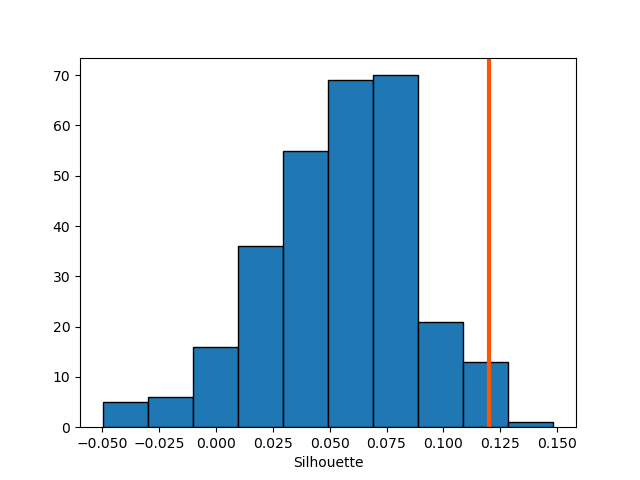
\includegraphics[width=\textwidth]{RandomSilhouetteDBSCAN_2.png}
\caption{Distribuzione della silhouette su $N_2$ per il sottoinsieme 2. Media: 0.06; Deviazione Standard: 0.03. La linea arancione rappresenta la silhouette sui dati reali.}
\label{etichetta2}
\end{minipage}
\end{figure}

\subsection{Hierarchical}
Per quanto riguarda il Hierarchical i sottoinsiemi che hanno mostrato i risultati migliori sono:

\begin{enumerate}
\item DistanceFromHome, Age, MonthlyIncome
\item PercentSalatyHike, TrainingTimeLastYear, MonthlyIncome, Age
\end{enumerate}

Per entrambi sono stati usati algoritmi di tipo agglomerativo con diverse definizioni della distanza inter clusters.
Ai fini della scelta del metodo da utilizzare, come primo approccio, si è deciso di visualizzare
lo scatter plot dei data frame alla ricerca di strutture che possano suggerire una scelta appropriata.
Dall' ananisi non sono emerse particolari evidenze e la decisione è ricaduta sui metodi che si sono rivelati più performanti.
Di seguito sono riportati i metodo usati per ciascun sottoinsieme e i rispettivi dendogrammi.

\begin{itemize}
\item Sottoinsieme 1: Group Average, Ward.
\item Sottoinsieme 2: Median, Ward.
\end{itemize}

\begin{figure}[H]
  \centering
  \begin{minipage}{.45\textwidth}
    \centering
    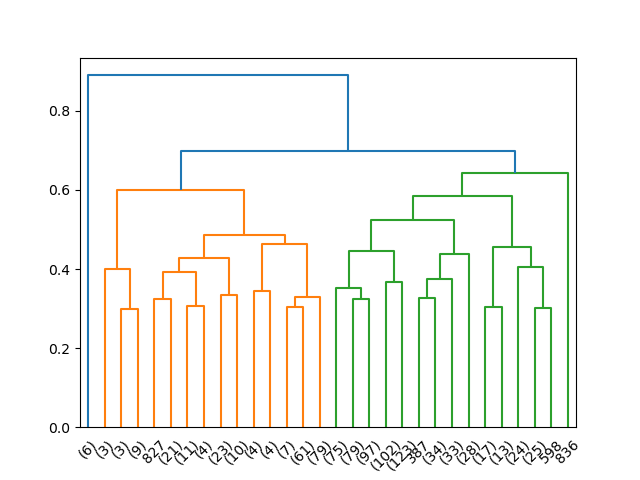
\includegraphics[width=\textwidth]{DistanceFromHome,Age,MonthlyIncome035Average.png}
    \caption{Dendogramma sottoinsieme 1:  metodo = Group Average;\\ silhouette = 0.35}
  \end{minipage}
  \begin{minipage}{.45\textwidth}
    \centering
    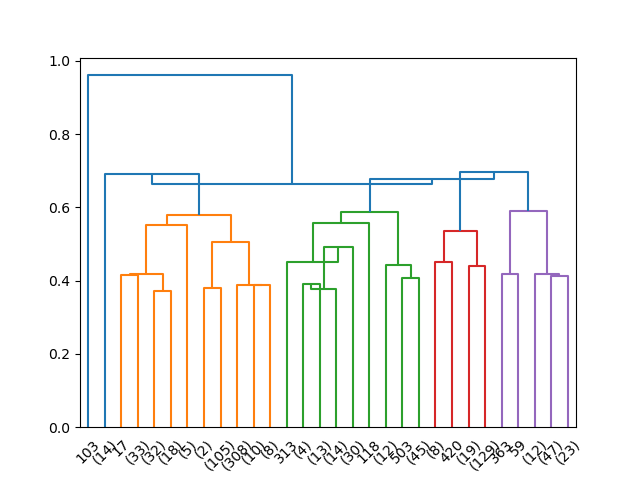
\includegraphics[width=\textwidth]{hierarchical_df3.png}
    \caption{Dendogramma sottoinsieme 2:  metodo = Median;\\ silhouette = 0.37}
  \end{minipage}
  \end{figure}

  \begin{figure}[H]
    \centering
    \begin{minipage}{.45\textwidth}
      \centering
      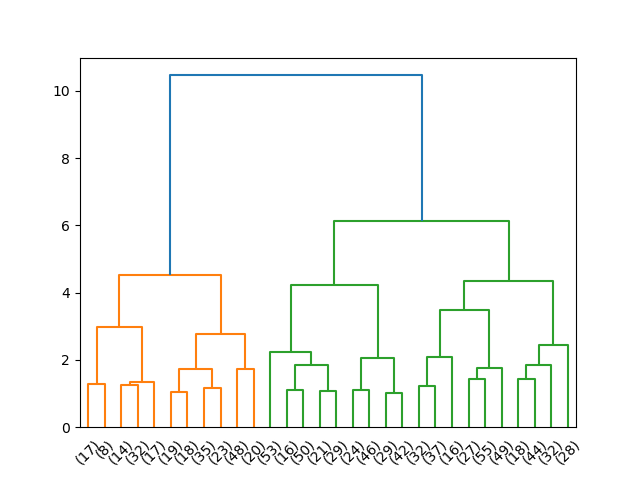
\includegraphics[width=\textwidth]{DistanceFromHome,Age,MonthlyIncome035Ward.png}
      \caption{Dendogramma sottoinsieme 1:  metodo = Ward;\\ silhouette = 0.35}
    \end{minipage}
    \begin{minipage}{.45\textwidth}
      \centering
      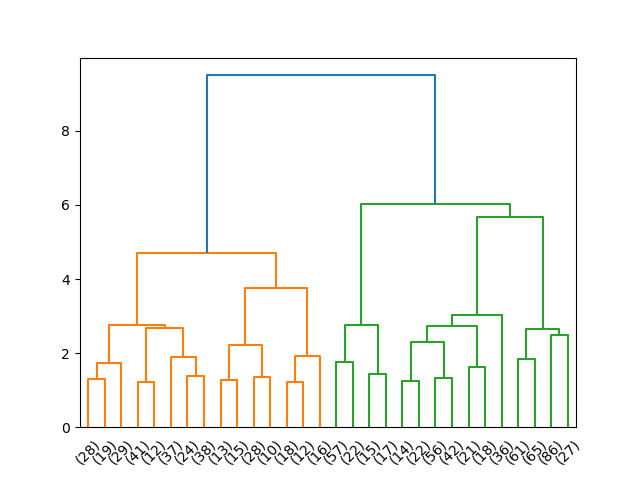
\includegraphics[width=\textwidth]{dendogram_hierarchicaldf3(ward).png}
      \caption{Dendogramma sottoinsieme 2:  metodo = Ward; \\silhouette = 0.24 }
    \end{minipage}
    \end{figure}


Nei dendogrammi mostrati è possibile notare le differenze dei vari metodi. In generale con Ward la robustezza risultante
è maggiore, sebbene nel secondo sottoinsieme la silhouette calcolata è significativamente più bassa rispetto all'altro metodo.

\subsubsection{Validazione}
Anche in questo caso per validare i risultati ottenuti, sono stati generati $N=500$ set di dati random su cui è stato eseguito l'algoritmo Hierarchical e calcolata la silhouette. Se quella valutata sui dati reali cade al di fuori della distribuzione (media $ \pm $ quattro deviazioni standard) allora il risultato è stato considerato attendibile.


\begin{figure}[H]
  \centering
  \begin{minipage}{.45\textwidth}
    \centering
    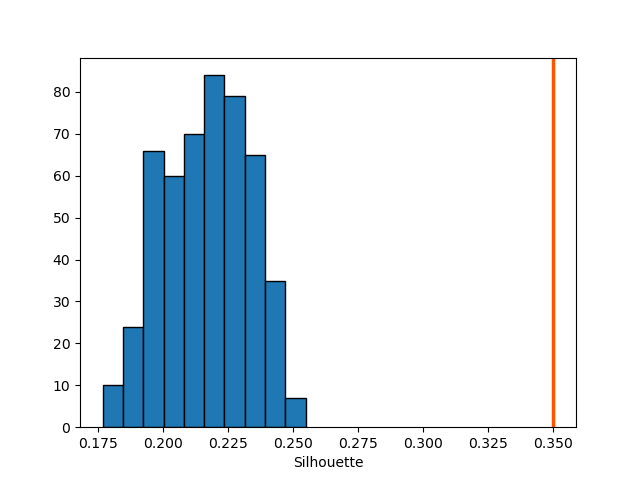
\includegraphics[width=\textwidth]{validation_hierDF1(ward).png}
    \caption{Distribuzione della silhouette su 500 set di dati random per il sottoinsieme 1. Media: 0.22; Deviazione Standard: 0.02. La linea arancione rappresenta la silhouette sui dati reali.}
  \end{minipage}
  \begin{minipage}{.45\textwidth}
    \centering
    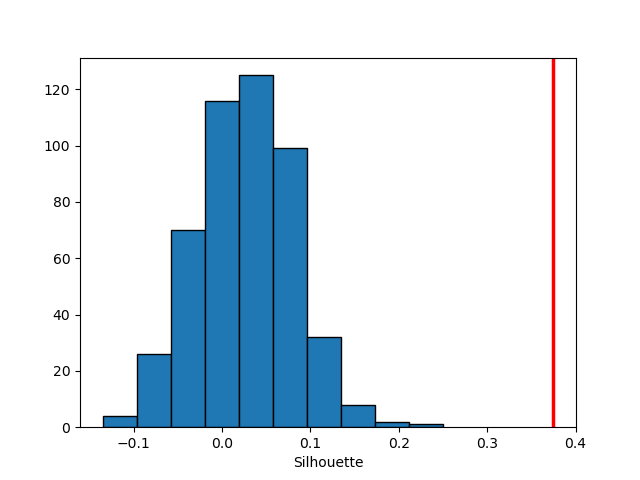
\includegraphics[width=\textwidth]{validation_silhouettehierdf2(median).png}
    \caption{Distribuzione della silhouette su 500 set di dati random per il sottoinsieme 1. Media: 0.03; Deviazione Standard: 0.08. La linea arancione rappresenta la silhouette sui dati reali. }
  \end{minipage}
  \end{figure}

% \begin{figure}[H]
%   \centering
%   \begin{minipage}{.45\textwidth}
%     \centering
%     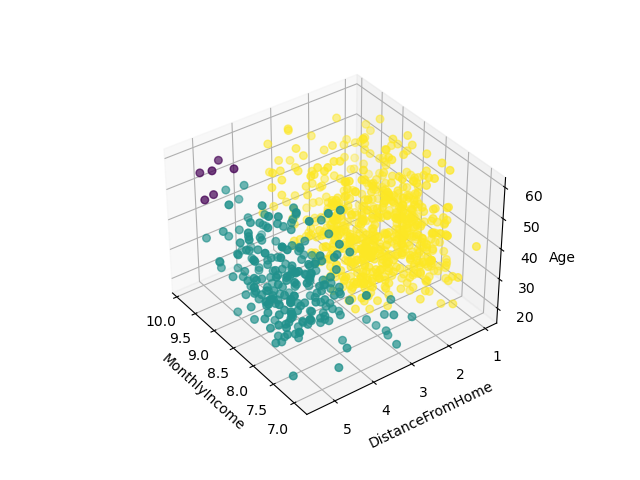
\includegraphics[width=\textwidth]{ScatterVisualPlotDF1_Hierarchical(Average).png}
%     \caption{Dendogramma sottoinsieme 2:  metodo = Median;\\ silhouette = 0.37}
%   \end{minipage}
%   \begin{minipage}{.45\textwidth}
%     \centering
%     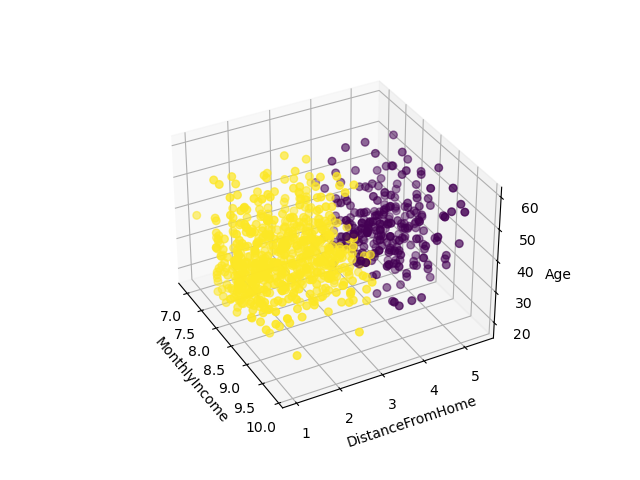
\includegraphics[width=\textwidth]{ScatterVisualPlotDF1_Hierarchical(Ward).png}
%     \caption{Dendogramma sottoinsieme 1:  metodo = Ward; \\silhouette = 0.35  }
%   \end{minipage}
%   \end{figure}

\subsection{Confronto fra gli algoritmi}
Alla luce di quanto ottenuto dai diversi algoritmi è possibile confrontare la bontà dei risultati ottenuti.\\
Sicuramente il DB-Scan è quello che ha avuto la resa peggiore, in quanto, come già precisato, soffre a causa della mancanza di variazioni significative di densità.\\
I risultati migliori in termini della silhouette sono relativi al K-Means e al Hierarchical. Inoltre, tramite quest'ultimo, è possibile scegliere il numero di clusters da utilizzare nel primo in modo da ottimizzare i risultati. Questo metodo è stato applicato per il seguente sottoinsieme 2 usato nel Hierarchical.
Ne è riportato lo scatter plot ricavato dal K-Means con $K=4$.
\begin{figure}[H]
    \centering
    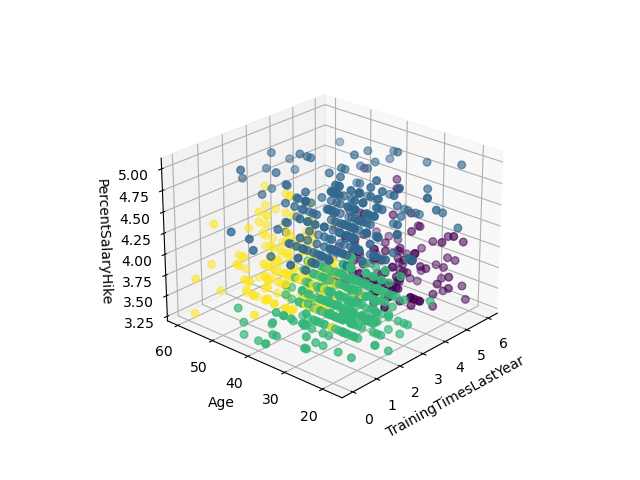
\includegraphics[scale=0.65]{FromHierarchicalKmeansDF2.png}
    \caption{Cluster sottoinsieme 2(par 4.3): SSE=96; silhouette=0.24 }
    \label{fig:my_label}
\end{figure}

I risultati sono nettamente migliori in termini dell'SSE.

\section{Classification}
Lo scopo in questo caso è quello di determinare modelli capaci di classificare i records presenti nel data frame in funzione dell'attributo Attrition. Sono stati usati due algoritmi differenti: Decision Tree e K-Nearest Neighbors. Per il primo il data frame considerato è stato quello precedente alla trasformazioni delle variabili, quindi senza missing values e con l'eliminazione del maggior numero di incongruenze possibili fra i dati. Ciò è stato fatto poiché la classificazione tramite Decision Tree non soffre se le distribuzioni dei dati sono sbilanciate e/o molto sparse. Per il secondo, invece, si è utilizzato il data frame con le variabili trasformate. 
In entrambi gli algoritmi i valori degli attributi categorici ordinali maggiormente correlati con Attrition (Tabella XXXX) sono stati stati sostituiti con valori numerici in maniera tale da ottenere una divisione binaria mantenendo l'ordinamento:

\begin{itemize}
\item Gender: 'Female'=0, 'Male'=1.
\item OverTime: 'No'=0, 'Yes'=1.
\item EnvironmentSatisfaction: 'Low'=0, 'Medium'=0, 'High'=1, 'Very High'=1.
\item WorkLifeBalance: 'Bad'=0, 'Good'=0, 'Better'=1, 'Best'=1.
\item JobInvolvement: 'Low'=0, 'Medium'=0, 'High'=1, 'Very High'=1.
\item MaritalStatus: 'Single'=0, 'Divorced'=0, 'Married'=1.
\end{itemize}

Siccome i valori dell'attributo Attrition sono fortemente sbilanciati a favore dei 'No' ($84\%$), si è deciso di effettuare un  random oversampling delle istanze relative al valore 'Yes' in modo da ridurre il bias presente nei dati. In particolare la frequenta del valore 'Yes' è passata dal $16\%$ al $23\%$ nel Decision Tree, mentre nel KNN dal $16\%$ al $20\%$.
Il data frame è stato suddiviso in train set ($70\%$) e test set ($30\%$). Inoltre ai fini della selezione del modello migliore è stata utilizzata la cross validation, in cui il train set è ulteriormente diviso in tre blocchi di cui due vengono usati per l'effettivo training ed uno, ciclicamente, per la validazione.

\subsection{Decision Tree}
Un classificatore di tipo $Decision Tree$ è caratterizzato da un diverso numero di parametri. Per la loro scelta è stata utilizzata la cross-validation in modo da ottenere la combinazione più performante degli stessi. 
I parametri scelti e il relativo range sono i seguenti:

\begin{itemize}
\item min impurity decrease $ \in [0,0.2]$: il minimo gain dell'impurità affinché il nodo venga splittato;
\item max depth $ \in [2,8]$: massima profondità dell' albero;
\item min samples split $ \in [2,8]$: numero minimo di valori di un nodo affinché esso venga splittato;
\item min samples leaf $ \in [2,8]$ :numero minimo di valori di un nodo affinché esso sia un  nodo leaf;
\item $\alpha$ $ \in [0,1]$: peso della complessità.
\end{itemize}

Le migliori combinazioni che ottimizzano rispettivamente la $Precision$ e la $Recall$ risultano essere:
\begin{itemize}
\item Precision: min impurity decrease$=0.0024$; max depth$=7$; min samples split$=5$; min samples leaf$=1$; $\alpha$=$0$.
\item Recall: min impurity decrease$=0.0$; max depth$=7$; min samples split$=3$; min samples leaf$=1$; $\alpha$=$0$.
\end{itemize}

Tali valori sono stati ulteriormente modificati per ridurre la complessità degli alberi generati sempre con lo scopo di migliorare le performance. Infatti, per come è stato implementata la cross-validation, Precision e Recall vengono ottimizzati singolarmente e quindi è possibile avere set di parametri maggiormente adatti agli scopi in esame che non erano stati indagati.
I modelli ottenuti sono:
\begin{itemize}
\item Modello 1: min impurity decrease$=0.0$; max depth$=8$; min samples split$=5$; min samples leaf$=2$; 
\item Modello 2: min impurity decrease$=0.0$; max depth$=3$; min samples split$=2$; min samples leaf$=1$; 
\item Modello 3: min impurity decrease$=0.001$; max depth$=12$; min samples split$=5$; min samples leaf$=1$; 
\item Modello 4: min impurity decrease$=0.003$; max depth$=6$; min samples split$=2$; min samples leaf$=1$; 
\end{itemize}

Di questi modelli sono state calcolate le rispettive ROC curve mostrate in Figura.NNNN
\begin{figure}[H]
    \centering
    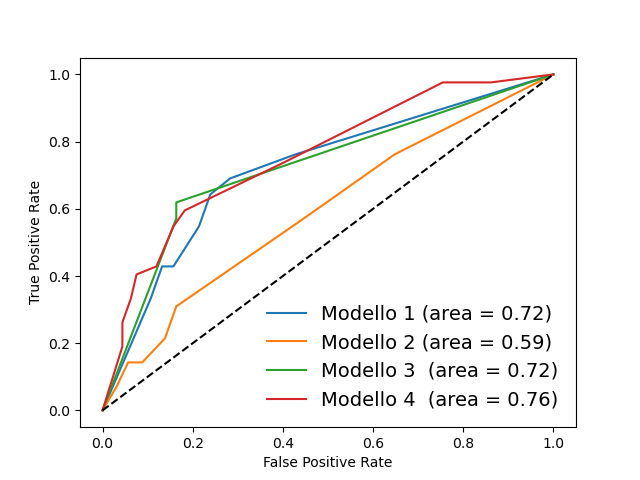
\includegraphics[scale=0.65]{ROC_CURVE.png}
    \caption{ROC curve dei quattro modelli selezionati.}
    \label{fig:my_label}
\end{figure}
Fra i quattro modelli, quello scelto è stato quello che ha presentato il valore dell'AUC maggiore, ovvero il Modello 4. Il corrispondente albero generato è il seguente

\begin{figure}[H]
    \centering
    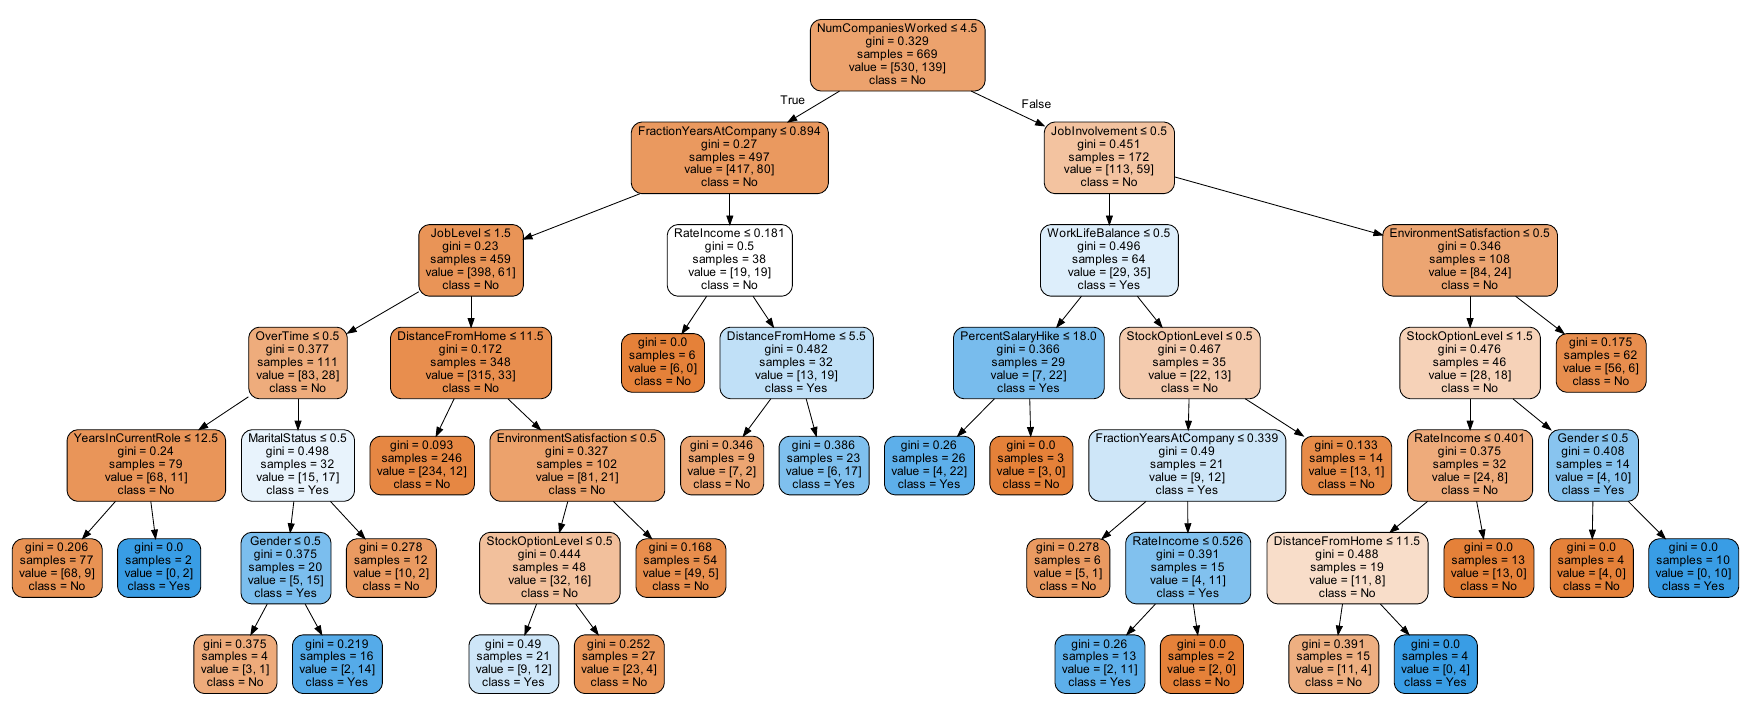
\includegraphics[scale=0.40]{Modello 4 (scelto).png}
    \caption{Decision tree generato dal Modello 4.}
    \label{fig:my_label}
\end{figure}

Applicando tale modello sul test set si sono ottenuti ricavati risultati che suggeriscono una buona performance del $Decision Tree$ selezionato.

\begin{figure}[H]
    \centering
\begin{tabular}{cc|cc}
\toprule
&\bfseries      & \multicolumn{2}{c}{\bfseries Predicted class} \\
& & \bfseries No & \bfseries Yes \\
\midrule
\bfseries Actual&\bfseries No  & 237 & 25  \\
\bfseries Class &\bfseries Yes & 31 & 37  \\
\bottomrule
\end{tabular}
\caption{Confusion Matrix del test set. 'No': Precision$=0.88$,\\ \qquad \qquad Recall$=0.90$; 'Yes': Precision$=0.60$, Recall$=0.54$}
\end{figure}

Come precedentemente detto, l'approccio dell'oversampling è stato utilizzato per ridurre il bias che il set di dati presentava a favore dei 'No' nell'attributo Attrition. Si verifica, infatti, che applicando le stesse procedure sul data frame originale i risultati che si ottengono sono nettamente peggiori, come si può notare dalla Confusion Matrix in Figura BOOOH.


\begin{figure}[H]
  \begin{minipage}{.45\textwidth}
    \centering
    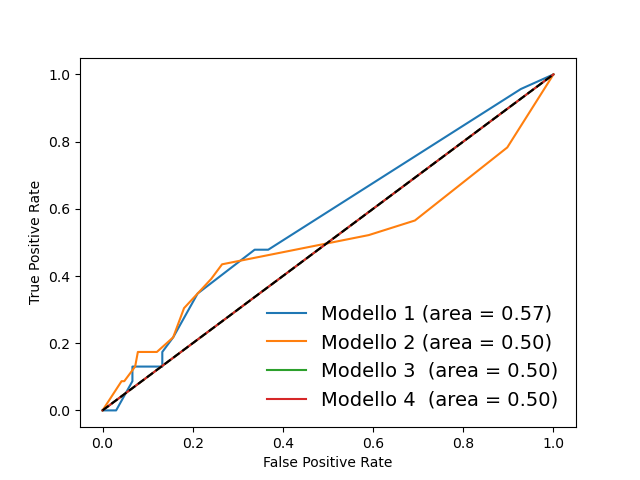
\includegraphics[width=\textwidth]{ROC_CURVEsenzaYes.png}
    \caption{ROC curve relativi a quattro modelli selezionati con il data frame originale.}
  \end{minipage}
  \centering
  \begin{minipage}{.45\textwidth}
       \centering
\begin{tabular}{cc|cc}
\toprule
&\bfseries      & \multicolumn{2}{c}{\bfseries Predicted class} \\
& & \bfseries No & \bfseries Yes \\
\midrule
\bfseries Actual&\bfseries No  & 231 & 7  \\
\bfseries Class &\bfseries Yes & 30 & 2  \\
\bottomrule
\end{tabular}
\caption{Confusion Matrix del test set. 'No': Precision$=0.89$, Recall$=0.97$; 'Yes': Precision$=0.22$, Recall$=0.06$}
  \end{minipage}

  \end{figure}







\subsection{K-Nearest Neighbors}
A differenza del caso precedente i dati sono stati normalizzati conservando la deviazione standard dei valori di partenza.
Gli unici parametri da dover scegliere in maniera opportuna sono il numero di primi vicini $k$ ed il peso da assegnare a ciascuno di essi relativamente alla loro distanza. Con lo scopo di ridurre l'impatto di $k$ sui risultati si è deciso di utilizzare come peso l'inverso del quadrato della distanza. Infatti, in tal modo, si da maggior importanza ai primi vicini più vicini.
Il range in cui si è fatto variare $k$ ai fini della massimizzazione delle performance del modello è stato $k \in [1,150]$. In seguito alla cross-validation, il miglior valore è risultato essere, come si può intuire dai grafici che seguono, $k=9$.

\begin{figure}[H]
  \centering
  \begin{minipage}{.45\textwidth}
    \centering
    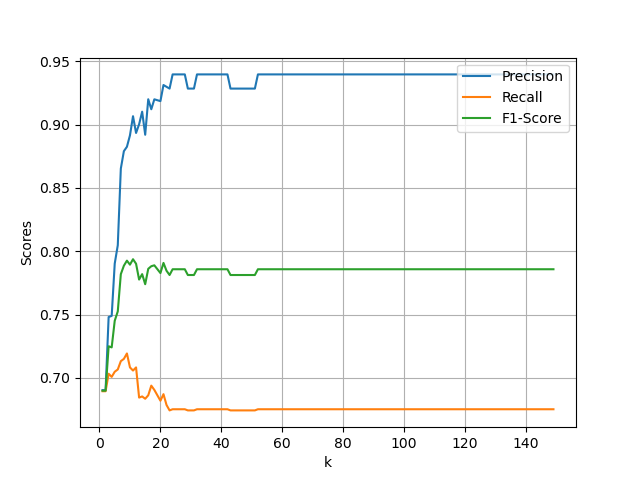
\includegraphics[width=\textwidth]{Gridsearch60distance.png}
    \caption{Risultati della cross-validation al variare del parametro $k$.}
  \end{minipage}
  \begin{minipage}{.45\textwidth}
    \centering
    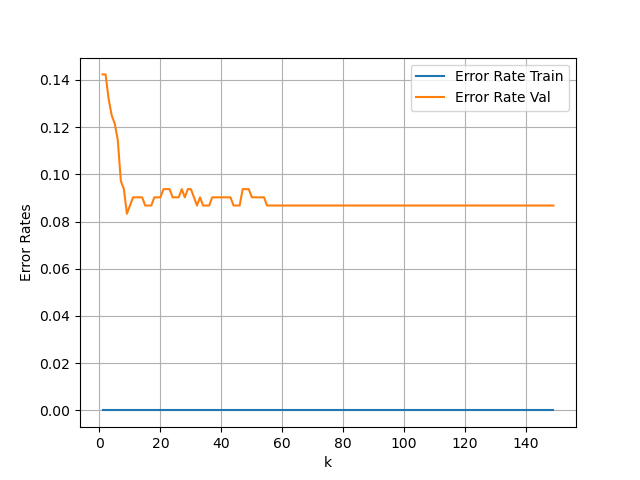
\includegraphics[width=\textwidth]{Overfitting60distance.png}
    \caption{Andamento dell'error rate sul train set e sul validation set. Si può notare l'overfitting del modello per piccoli valori di $k$.}
  \end{minipage}
  \end{figure}
In Figura XXXsx si evince come il compromesso migliore fra i tre scores risulta essere $k=8$, dove si nota il massimo dell'F1-Score che quindi rappresenta un buon bilanciamento fra Precision e Recall. Questo valore corrisponde anche al minimo del validation error rate in Figura XXXdx.
Di seguito è riportato il risultato del modello selezionato sul test set, tramite la Confusion Matrix.\\

\begin{figure}[H]
    \centering
\begin{tabular}{cc|cc}
\toprule
&\bfseries      & \multicolumn{2}{c}{\bfseries Predicted class} \\
& & \bfseries No & \bfseries Yes \\
\midrule
\bfseries Actual&\bfseries No  & 235 & 3  \\
\bfseries Class &\bfseries Yes & 21 & 29  \\
\bottomrule
\end{tabular}
\caption{Confusion Matrix del test set. Precision=0.91, Recall=0.58}
\end{figure}
Si può notare come, sebbene l'approccio dell'oversampling abbia sanato parzialmente lo squilibrio fra i due valori di Attrition, resta comunque un bias in favore dei 'No'.

\section{Association Rules}
Lo scopo è quello di ricavare le $Association Rules$ più interessanti nei dati disponibili. Poichè il numero degli itemsets e di consegeuenza il numero delle regole cresce esponenzialmente al variare dei valori, sono stati scartati gli attributi considerati meno importanti, ovvero:
'PerformanceRating', 'TrainingTimesLastYear', 'StockOptionLevel',  'YearsInCurrentRole',  'NumCompaniesWorked','PercentSalaryHike',  'OverTime',  'RateIncome', 'FractionYearsAtCompany'.\\
L'unico attributo numerico continuo sopravvissuto, 'DistanceFromHome', è stato categorizzato in $10$ valori tramite la suddivisione in intervalli.
Parte della suddivisione dei data frame.
Come prima cosa sono stati determinati gli itemsets più frequenti, i massimali e i chiusi al variare del valore minimo del supporto. Come si può osservare dal grafico in Figura XXXXX all'aumentare del supporto minimo il numero degli itemset descresce velocemente, in particalore seguono un andamento esponenziale decrescente.

\begin{figure}[H]
    \centering
    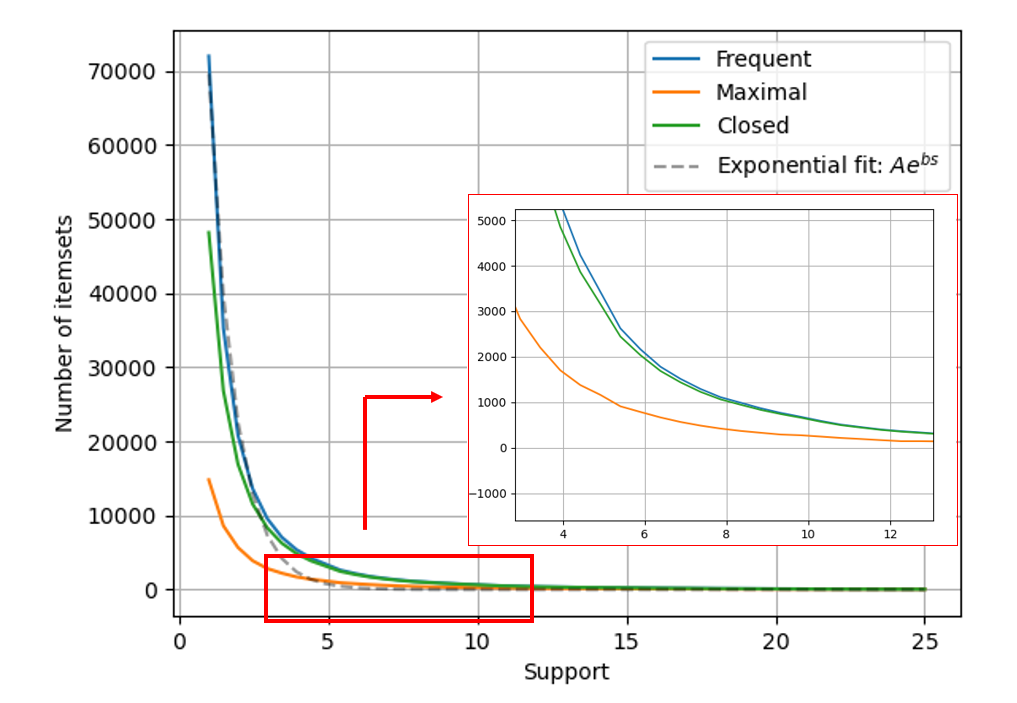
\includegraphics[scale=0.65]{Frequen,_maximal_and_closed_itemsets da inserire.png}
    \caption{Numero dei diversi tipi di itemsets in funzione del supporto minimo.\\Valori del fit: $A=219226$ ; $s=-1.15$. }
    \label{fig:my_label}
\end{figure}

Successivamente si è valutato il numero di rules in funzione della confidence per diversi valori del supporto minimo. Come ci si poteva aspettare il numero di regole trovate diminuisce all'aumentare della confidence e del supporto minimo.

\begin{figure}[H]
    \centering
    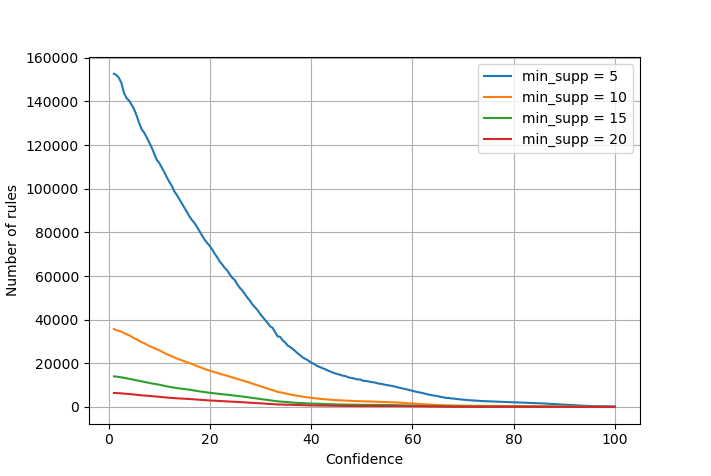
\includegraphics[scale=0.65]{Confidence_figure.png}
    \caption{Numero delle regole in funzione della confidence per $4$ diversi valori del supporto minimo.}
    \label{fig:my_label}
\end{figure}

Per le fasi seguenti è stato scelto come supporto il valore $10$ per avere un numero consono ($633$) di itemsets da analizzare.
Come misura di interesse per ciascuna regola è stato utilizzato l'$Interest Factor$ ('$lift$'), di seguito è presentato l'istogramma del numero delle regole al variare del lift.  

\begin{figure}[H]
    \centering
    \includegraphics[scale=0.70]{lifthistogram.png}
    \caption{Istogramma del numero delle regole al variare del $lift$' per $3$ valori della confidence: $30\%$; $50\%$; $70\%$}
    \label{fig:my_label}
\end{figure}

Di conseguenza le regole più interessanti scelte risultano essere quelle con lift maggiore di $3$ siccome il numero di regolore significativamente  minore di $1$ è nullo. Le regole selezionate risultano essere:

\begin{enumerate}
\item ($3.0$, 'Research and Development', 'No') $\longrightarrow$ 'Research Director'
\item ($1.0$, 'Life Science', 'Research and Development') $\longrightarrow$ 'Research Scientist'
\item ('Sales', $2.0$, 'Better\_WorkLifeBalance') $\longrightarrow$ 'Sales Executive'
\item ('Sales', $2.0$, 'No') $\longrightarrow$ 'Sales Executive'
\end{enumerate}

Fra queste, quelle ulteriormente indagate sono state la $1$ e la $3$.
Di seguito sono mostrate le tabelle di contigenza relatice alle due regole usate per la sostituzione dei missing value

\begin{figure}[H]
  \centering
  \begin{minipage}{.45\textwidth}
    \centering
    \begin{tabular}{l|cc|r}
& \bfseries B & \bfseries nonB &\\
\hline
\bfseries A & 3 & 27 &30\\
\bfseries nonA & 0&10&10\\
\hline
& 3&37&40\\
\end{tabular}
    \caption{tabella di contingenza regola 1}
  \end{minipage}
  \begin{minipage}{.45\textwidth}
    \centering
    \begin{tabular}{l|cc|r}
& \bfseries B & \bfseries nonB &\\
\hline
\bfseries A & 28& 2 &30\\
\bfseries nonA & 0&56&56\\
\hline
& 28&58&86\\
\end{tabular}
    \caption{tabella di contigenza regola 3.}
  \end{minipage}
  \end{figure}



%\section{Conclusioni}
\end{document}

